% =====================================================================
%  draft.tex — Score-Bundle Models: the thesis draft.
%
%  The full model derivation is folded into Chapter~\ref{ch:model}
%  (merged from the early standalone formulation note, since deleted).
%
%  Prose is written wherever the result is known and honest.  \TODO{...}
%  marks the few genuinely open items (final figures, personal/title
%  details).  Exact figures live in docs/graphgp_first_design.md (primary),
%  docs/phase1_calibration_results.md and docs/downstream_tasks_results.md
%  (two-stage development record).
%
%  Compiles with plain pdflatex (no bibtex — manual thebibliography).
%  Headline numbers are centralised in the macros below: ONE place to edit.
% =====================================================================
\documentclass[11pt,a4paper]{report}

\usepackage[utf8]{inputenc}
\usepackage[T1]{fontenc}
\usepackage[margin=1in]{geometry}
\usepackage{amsmath,amssymb,amsthm,bm}
\usepackage{graphicx}
\usepackage{booktabs}
\usepackage{longtable}
\usepackage{array}
\usepackage{xcolor}
\usepackage{enumitem}
\usepackage[hidelinks]{hyperref}

\graphicspath{{figures/}}
\setlength{\emergencystretch}{3em}  % absorb the odd overfull line gracefully

% --- draft helpers ---------------------------------------------------
\newcommand{\TODO}[1]{{\color{red}\textbf{[TODO: #1]}}}
\newcommand{\placeholder}[1]{{\color{gray}\textit{#1}}}
% Figure placeholder: shows the figure if present, else a TODO box.
\newcommand{\figph}[3]{% {file}{width}{caption}
  \begin{figure}[t]\centering
  \IfFileExists{figures/#1}{\includegraphics[width=#2\linewidth]{#1}}%
    {\fbox{\parbox[c][0.28\linewidth][c]{#2\linewidth}{\centering\TODO{missing figure: \texttt{\detokenize{#1}}}}}}
  \caption{#3}\end{figure}}

% --- DEVELOPMENT-set numbers (30 pieces; used for all model selection) ----------
% two-stage pipeline rows (docs/phase1_calibration_results.md, strict protocol)
\newcommand{\rmseZero}{0.566}
\newcommand{\rmseGraph}{0.404}
\newcommand{\rmseNetGraph}{0.393}      % music-model mean + plain graph (development, strict)
\newcommand{\rmseStack}{0.388}         % features + music-model mean + plain graph (development, strict)
\newcommand{\rmseHeadline}{0.379}      % two-stage-era headline: feat+net+harmonic graph (development; superseded by \rmseGP)
\newcommand{\nllHeadline}{$-0.346$}
\newcommand{\nllZero}{$-0.007$}
\newcommand{\nllGraph}{$-0.308$}
\newcommand{\nllNetGraph}{$-0.322$}
\newcommand{\nllStack}{$-0.333$}
\newcommand{\covZero}{87\%}
\newcommand{\covHead}{92\%}            % coverage of nominal-90\% intervals
\newcommand{\nPieces}{30}
\newcommand{\maskRate}{40\%}
\newcommand{\rmseNetOff}{0.446}        % music-model mean, graph off (strict: logs/maskaware.log music model-ma off)
\newcommand{\nllNetOff}{$-0.164$}
\newcommand{\covNetOff}{90\%}
% proposed model, development set (logs/graphgp_v2_report.log, a single code version)
\newcommand{\rmseGPdev}{0.360}
\newcommand{\nllGPdev}{$-0.404$}
% --- CONFIRMATION-set numbers (20 untouched pieces, preregistered, run ONCE) -----
% logs/confirmation_verdict.log
\newcommand{\nConfPieces}{20}
\newcommand{\rmseGP}{0.376}            % THE headline: proposed model on confirmation
\newcommand{\nllGP}{$-0.300$}
\newcommand{\covGP}{92.5\%}
\newcommand{\rmseConfOldHead}{0.393}   % two-stage-era headline on confirmation
\newcommand{\nllConfOldHead}{$-0.311$}
\newcommand{\dRmseConf}{$-0.014$}      % paired, proposed model vs. strongest two-stage configuration, RMSE (sig.)
\newcommand{\dNllGraphConf}{$-0.074$}  % paired graph contribution inside proposed model, NLL (sig.)

% --- notation (must match CLAUDE.md's canonical table) ----------------
\newcommand{\R}{\mathbb{R}}
\newcommand{\N}{\mathcal{N}}
\newcommand{\score}{\mathcal{S}}
\newcommand{\graph}{\mathcal{G}}
\newcommand{\Qg}{Q_{\graph}}
\newcommand{\Lg}{L_{\graph}}
\newcommand{\muLM}{\mu_{\mathrm{LM}}}  % music-model prior mean
\newcommand{\Sy}{\Sigma_y}             % posterior covariance
\newcommand{\diag}{\operatorname{diag}}

\title{\textbf{Score-Bundle Models}\\[0.3em]
  \large Bayesian Score-Informed Performance Transcription
  with Calibrated Uncertainty}
\author{Raynaldi Lalang \\[0.5em]
  \small Supervisor: Kazuyoshi Yoshii \\
  \small Kyoto University}
\date{Thesis draft --- compiled \today}

\begin{document}
\maketitle

\begin{abstract}
\noindent Given a printed score and a recording of a performance (as piano MIDI in
this work), we recover \emph{how} each written note was played --- its
micro-timing, articulation, and dynamics --- together with a calibrated statement
of confidence. The model is \textbf{one multi-output Gaussian process on the score
graph}: notes related in the score are related in performance (a graph GP in the
sense of Borovitskiy et al.), the three expressive channels are coupled by a
coregionalization matrix, and all side information --- hand-built score features
and per-note embeddings from a small, from-scratch symbolic music language model
(hereafter the \emph{music model})
--- enters as linear kernels, i.e.\ as a marginalized Bayesian linear mean. One
exact marginal likelihood per piece learns every hyperparameter. Development used
\nPieces{} held-out ASAP pieces; the headline claims were then \emph{preregistered
and confirmed exactly once} on \nConfPieces{} further pieces untouched by any
modelling decision: the model recovers hidden notes with lower error than the
strongest \emph{two-stage} pipeline it subsumes --- a plug-in mean followed by a
graph GP on the residual (RMSE~\rmseGP{} vs.\ \rmseConfOldHead,
paired difference \dRmseConf{} significant), the graph's contribution to
calibration is confirmed (paired NLL \dNllGraphConf), and nominal-90\% intervals
cover $\approx\covGP$ of the truth. Six downstream tasks map where the structure
helps (per-note recovery, confidence, error spotting) and where it does not
(whole-performance summaries; extrapolation from a short excerpt, where a
cross-piece head remains the honest tool). Phase~2 carries the same prior,
unchanged, to intonation, vibrato, loudness, timing, and vibrato onset delay
on continuously pitched
instruments: on real recordings (URMP, development set) the full pipeline ---
tracker, per-note estimator, onset-anchored warp, per-(note, channel)
missingness, heteroscedastic
likelihood --- runs end to end on a six-channel bundle; the graph prior
significantly improves recovery on intonation and vibrato and calibration on
vibrato and timing (the vibrato-extent calibration star is seed-sensitive),
with coverage on target on every channel; the registered claim set was then
\emph{confirmed in a single one-shot} on the frozen 13-piece pool ---
intonation recovery, vibrato calibration on both channels, coverage on all six
channels; the secondary timing-calibration claim failed and is reported
verbatim. Phase~3 (audio via a differentiable
synthesizer) is scoped but not built.
\end{abstract}

\tableofcontents

% =====================================================================
\chapter{Introduction}\label{ch:intro}

\section{Motivation}
A score specifies \emph{what} to play; a performance realises \emph{how}. The
difference --- micro-timing, articulation, dynamics --- is where musical expression
lives, and recovering it from a recording is both scientifically interesting and
practically useful (analysis, pedagogy, expressive rendering, and as structured
supervision for audio models). Two commitments shape the whole thesis. First, the
score is treated as \emph{known}: we solve the inverse of expressive synthesis, not
full transcription. Second, \emph{uncertainty is a primary output}: a per-note
estimate is only actionable with a calibrated error bar, and calibration is
evaluated as rigorously as accuracy.

\section{Problem statement}
Let a symbolic score fix, for each note, its pitch, score onset, and notated
duration. A performance assigns to each note a small vector of continuous
expressive variables --- here onset residual $\tau$, log articulation ratio
$\log r$, and normalised velocity $v$. Given the score and an aligned performance,
the task is to infer the posterior over these per-note variables, including for
notes that are held out (masked), and to do so with calibrated uncertainty. This is
\emph{score-informed performance transcription} (equivalently, probabilistic
inverse synthesis). Inferring the score itself (full automatic music transcription)
is out of scope; see \S\ref{sec:scope} and \S\ref{sec:future-amt}. The central
empirical question is:
\begin{quote}
\itshape Does a score-structured prior improve expressive-variable recovery
\emph{and} uncertainty calibration compared with independent or purely temporal
baselines?
\end{quote}
A \emph{win} is defined before any test number is seen, and requires improvement on
\emph{both} axes at once (\S\ref{sec:metrics}).

\section{Terminology: the proposed model and the two-stage pipeline}\label{sec:twostage}
Two names recur throughout. \textbf{The proposed model} is the thesis model: one
multi-output Gaussian process over all notes and all three expressive channels, in
which the score graph, the hand-built score features, and the music model's per-note
representation all enter a single kernel, and every hyperparameter is learned from
one per-piece marginal likelihood (\S\ref{sec:gpfirst}). \textbf{The two-stage
pipeline} is the earlier system it subsumes and is compared against: a \emph{plug-in
mean} --- a point estimate of each note's expression, fitted once across pieces from
the features and the music model --- followed by a \emph{separate} graph GP fitted to
the residual, one scalar GP per channel. Its numbers are the development record;
formally it is a special case of the proposed model, recovered by fixing the
coregionalization to be diagonal, the graph parameters to constants, and the mean to
a plug-in estimate, and the equality is pinned by unit tests (\S\ref{sec:special-cases}).

\section{Contributions}
\begin{enumerate}[leftmargin=*]
  \item \textbf{A multi-output graph Gaussian process for expressive performance}
        (\S\ref{sec:gpfirst}): channels coupled by coregionalization, a spectral
        kernel of the score-graph Laplacian, and all side information ---
        hand-built score features and learned music-model embeddings --- entering
        as marginalized Bayesian linear means; every hyperparameter learned by the
        exact per-piece evidence, posterior and calibration in closed form. Its
        claims were \textbf{preregistered and confirmed once} on evaluation pieces
        untouched by any modelling decision.
  \item \textbf{Measured attribution} (\S\ref{sec:attribution}): per-piece Bayesian
        weighting of informative features does the recovering; the graph makes the
        confidence honest (its calibration contribution independently confirmed);
        the from-scratch music model earns its place as a feature provider inside the
        kernel --- each claim isolated by nested ablations, including the entire
        two-stage development pipeline as a provable special case.
  \item \textbf{A map of where the structure helps}, via six downstream tasks with
        objective metrics, re-validated under the final model, yielding two crisp
        boundaries (\S\ref{sec:boundary}): structure helps note-level judgments,
        not whole-performance summaries; per-piece adaptation helps interpolation,
        not excerpt extrapolation.
  \item \textbf{Methodological rigour as a result in its own right}: a discovered
        and fixed evaluation leak pinned by structural tests and bitwise
        end-to-end audits, a strict leakage-free protocol, contamination
        filtering, self-validating robustness safeguards, and a
        development/confirmation split that caught selection inflation in the act
        (\S\ref{sec:hygiene}).
  \item \placeholder{(Planned / future)} A path to audio via a
        differentiable-synthesizer likelihood (Phase~3) and a geometric
        ``connection-Laplacian'' generalisation of the graph prior.
\end{enumerate}

\section{Scope and non-goals}\label{sec:scope}
In scope (Phase~1): piano; symbolic (MIDI) performance variables --- onset timing
$\tau$, articulation $\log r$, dynamics $v$; known score support (note identities,
score onsets, score durations); held-out evaluation with calibration.

\noindent\textbf{Explicit non-goals for the first version:}
\begin{itemize}[leftmargin=*,noitemsep]
  \item discovering unknown score support from audio (that is full AMT --- a future
        extension, \S\ref{sec:future-amt});
  \item performer-controlled intonation or timbre \emph{from piano} (these do not
        exist on a fixed-pitch keyboard);
  \item arbitrary instruments and room acoustics;
  \item any claim that the model performs general automatic music transcription.
\end{itemize}
Audio input/output and continuously pitched instruments enter only in Phases~2--3.
The work is phased so that each stage produces a defensible result before the next
risk is taken (Table~\ref{tab:phases}); Phase~0 (the from-scratch music model) and
Phase~1 (the score-graph prior and its evaluation) are complete, Phase~2 has
development-set results on real recordings with its confirmation set frozen but
not yet spent, and Phase~3 is scoped and not built.

\begin{table}[h]\centering
\caption{The four phases and their status.}
\label{tab:phases}
\footnotesize
\begin{tabular}{@{}p{1.6cm}p{4.5cm}p{4.2cm}p{3.2cm}@{}}
\toprule
Phase & Scope & Adds & Status \\
\midrule
0 --- foundation & From-scratch symbolic music model (backbone + representations) &
Per-note embeddings $h_i$ (a feature kernel of the Phase-1 GP; the plug-in mean $\muLM$ of the two-stage baseline) & \textbf{Done} \\
1 --- core (piano) & Timing, articulation, dynamics from aligned score+performance &
Score-graph GMRF prior, closed-form posterior, calibrated uncertainty &
\textbf{Done}; result in and hardened \\
2 --- extension (mono) & Intonation, vibrato, loudness on continuously pitched instruments &
$f_0$-derived channels ($c_i$ cents, vibrato, $\ell_i$) $+$ $\tau$, $\delta^{\mathrm{vib}}$ & \textbf{Confirmed} (URMP; registered one-shot on the frozen 13-piece pool): intonation recovery, vibrato calibration on both channels, coverage on all six channels; the secondary timing-calibration claim failed, reported verbatim \\
3 --- extension (waveform) & Differentiable synthesizer as audio likelihood &
Harmonic amplitudes $a$, audio $x$ & Scoped; conjugate helpers tested; first single-note waveform-likelihood inference demonstrated on real audio (development, exploratory) \\
\bottomrule
\end{tabular}
\end{table}

\section{Thesis outline}
Chapter~\ref{ch:related} positions the work against expressive-performance
modelling, alignment, structured priors, symbolic music models, and differentiable
synthesis. Chapter~\ref{ch:model} gives the complete model and derivation.
Chapter~\ref{ch:data} describes the data and the evaluation protocol, including
contamination control. Chapter~\ref{ch:results} reports the Phase-1 result and the
methodological findings. Chapter~\ref{ch:downstream} maps the downstream reach.
Chapters~\ref{ch:discussion}--\ref{ch:conclusion} discuss, situate, and conclude;
appendices hold the notation summary and additional tables.

% =====================================================================
\chapter{Background and Related Work}\label{ch:related}

\section{Computational models of expressive performance}
Expressive-performance research models how performers deviate from the notated
score in timing, dynamics, and articulation, historically with rule-based systems
and, more recently, with sequence models trained on aligned corpora
\cite{cancino2018,oore2018}. Most such work predicts a single expressive rendering
or studies aggregate statistics. This thesis differs in framing the problem as
\emph{per-note Bayesian inference with calibrated uncertainty}, and in asking not
only how accurately expression can be predicted but how \emph{trustworthy} the
per-note confidence is.

\section{Score-to-performance alignment}
Aligned corpora pair a symbolic score with a performance via a note- or beat-level
correspondence, from which continuous deviations can be read off. ASAP provides
score$\leftrightarrow$performance alignments for piano with beat and downbeat
annotations \cite{asap}, and is the source of the targets used here. The quality of
this alignment upper-bounds the quality of the extracted targets, a dependence we
treat as an explicit limitation (Chapter~\ref{ch:discussion}).

\section{Structured priors: graph Gaussian processes, GMRFs, and the SPDE approach}
Gaussian Markov random fields place a Gaussian prior whose sparse precision encodes
conditional-independence structure \cite{rueheld2005}. The SPDE approach links
Gaussian fields to GMRFs and yields Mat\'ern-type priors with interpretable range
and smoothness \cite{lindgren2011}; these constructions extend to graphs, giving
Mat\'ern \emph{Gaussian processes on graph nodes} \cite{borovitskiy2021}. For
vector-valued outputs, both the intrinsic-coregionalization construction of
\cite{borovitskiy2021} and the Kronecker output-coupling of Gaussian processes over
graphs \cite{venkitaraman2018} prescribe an explicit cross-output covariance;
GPs on \emph{evolving} graphs \cite{blancomulero2021} address dynamic structure,
which a fixed score does not need. Our model is exactly such a multi-output graph
Gaussian process --- the graph kernel a spectral function of the score-graph
Laplacian, channels coupled by a coregionalization matrix, side information
marginalized into the kernel as Bayesian linear means, and every hyperparameter
learned by the exact evidence --- with the graph built from musical adjacency
rather than physical space.

\section{Symbolic music language models}
Transformer and RNN models over tokenised MIDI (Music Transformer, REMI,
performance RNNs) learn strong distributions over symbolic music
\cite{musictransformer,remi,oore2018}. We build a small decoder-only model from
scratch (in the spirit of nanoGPT \cite{nanogpt}) rather than downloading a
pretrained one, so that the uncertainty layer can attach to its internals and the
calibration and leakage claims remain inspectable and honest.

\section{Differentiable synthesis}
Differentiable digital signal processing renders audio from interpretable controls
(fundamental frequency, harmonic amplitudes, noise) through a differentiable
synthesizer \cite{ddsp}. This is the intended Phase-3 likelihood: it connects the
latent performance variables to a waveform while keeping the amplitudes
conditionally Gaussian, so they can be marginalised in closed form
(\S\ref{sec:phase3-math}).

% =====================================================================
\chapter{Model and Formulation}\label{ch:model}
\emph{This chapter gives the complete model derivation. Notation is summarised in
Appendix~\ref{app:notation}.}

\section{Setting}
A \emph{score} is the known discrete support
\begin{equation}
  \score = \{ s_i \}_{i=1}^{N}, \qquad s_i = (p_i,\, b_i,\, d_i),
  \label{eq:support}
\end{equation}
where $p_i$ is the pitch (MIDI number), $b_i \ge 0$ the onset in score time
(beats), and $d_i > 0$ the notated duration (beats). A \emph{performance} attaches
to each score event a vector of continuous expressive variables; in Phase~1
(piano),
\begin{equation}
  y_i \;=\; \bigl[\, \tau_i,\; \log r_i,\; v_i \,\bigr] \in \R^{3},
  \label{eq:variables}
\end{equation}
defined relative to the monotone score-time warp $T(\cdot)$ (score beats $\to$
performance seconds). The warp is read off the alignment: the local tempo, in seconds
per beat, is estimated by finite differences of performed time against score time
along the aligned beat grid, and $T$ is its cumulative integral over score time, so
that $T(b)$ is the tempo-implied arrival of beat $b$. $T$ is estimated from
the same performance's aligned beat grid and then treated as known; its
estimation error is not propagated (a limitation Phase~2 addresses
explicitly with a leave-one-out warp, \S\ref{sec:phase2}). Conditional on $T$, the three
channels are
\begin{align}
  \tau_i   &= t_i - T(b_i), \label{eq:tau}\\
  \log r_i &= \log \frac{\delta_i}{\,T(b_i + d_i) - T(b_i)\,}, \label{eq:logr}\\
  v_i      &= \tilde v_i / 127 - \overline{\tilde v/127}. \label{eq:vel}
\end{align}
Here $\tau_i$ is the \emph{onset residual} in seconds (performed onset $t_i$ minus
the tempo-implied onset $T(b_i)$); $\log r_i$ is the \emph{articulation} (log ratio
of performed duration $\delta_i$ to the warp-implied duration); and $v_i$ is the
\emph{dynamics} (centred, unit-range MIDI velocity $\tilde v_i$). Conditioning on
the warp $T$ is what makes the per-note field $y$ well defined and jointly Gaussian.
Later phases add channels on
the same support: intonation $c_i$ (cents), vibrato parameters, and the fundamental
curve $f_0$ (Phase~2); harmonic amplitudes $a$ (Phase~3). Not every variable is
available, measurable, or even meaningful on every instrument; Table~\ref{tab:variables}
is honest about this --- piano gives reliable timing, articulation, and dynamics
but \emph{no} performer-controlled intonation, which is why intonation and
vibrato wait for continuously pitched instruments. The task is
\emph{score-informed}: $\score$ is given, and we infer the posterior over $y$
(inverse direction) from observations generated by the same model that, run
forward, synthesises a performance.

{\footnotesize
\begin{longtable}{@{}p{3.1cm}p{2.0cm}p{2.0cm}p{0.9cm}p{4.4cm}@{}}
\caption{Performance variables by phase, with what they are realistic for.}
\label{tab:variables}\\
\toprule
Variable & Symbol & Unit & Phase & Realistic for \\
\midrule
\endfirsthead
\toprule
Variable & Symbol & Unit & Phase & Realistic for \\
\midrule
\endhead
\bottomrule
\endfoot
Score-time warp (local tempo) & $T(\cdot)$ & s/beat, integrated & 1 & all (defines the score$\to$time warp) \\
Note onset residual & $\tau_i$ & s (report ms) & 1 & all \\
Articulation / duration ratio & $\log r_i$ & dimensionless & 1 & all (esp.\ piano) \\
Velocity / dynamics & $v_i$ & norm.\ MIDI & 1 & keyboard reliable; others approximate \\
Intonation deviation & $c_i$ & cents & 2 & voice, strings, winds --- \emph{not} piano \\
Instantaneous $f_0$ curve & $f_{0,i}(t)$ & Hz & 2 & monophonic pitched \\
Vibrato (rate, extent, delay) & $f_i^{\mathrm{vib}}, \gamma_i, \delta_i^{\mathrm{vib}}$ & Hz, cents, s & 2 & voice, strings, winds \\
Loudness (audio) & $\ell_i$ & log RMS & 2 & monophonic pitched \\
Amplitude envelope & $A_i(t)$ & normalised & 2--3 & monophonic \\
Harmonic amplitudes / timbre & $\mathbf a_i$ & --- & 3 & narrow / monophonic only \\
Posterior uncertainty & $\sigma_i$ / CI & same as variable & all & all \\
\end{longtable}}

\section{The score graph}
Let $\graph = (V, E)$ be a weighted graph on the $N$ score events with
Gaussian-kernel edge weights
\begin{equation}
  W_{ij} \;=\; \exp\!\Bigl( -\tfrac{(b_i - b_j)^2}{2\,\ell_b^2} - \tfrac{(p_i - p_j)^2}{2\,\ell_p^2} \Bigr)
  \;+\; w_v\, \mathbf{1}[\text{voice}_i = \text{voice}_j],
  \qquad W_{ii} = 0,
  \label{eq:adjacency}
\end{equation}
with length scales $\ell_b$ (beats) and $\ell_p$ (semitones) and an optional
same-voice bonus $w_v \ge 0$. Throughout, these are untuned defaults:
$\ell_b = 2$, $\ell_p = 4$, $w_v = 0$. ASAP carries no voice labels, so the
voice bonus is inert in every reported run and stands as the documented
hook for voiced corpora. The (combinatorial) graph Laplacian is
\begin{equation}
  \Lg \;=\; D - W, \qquad D = \diag\Bigl(\textstyle\sum_j W_{ij}\Bigr).
  \label{eq:laplacian}
\end{equation}
The \emph{temporal-only} baseline replaces $W$ by the chain adjacency of score-time
order (each note coupled only to its temporal neighbours), an AR(1)-style smoother;
the \emph{independent} baseline drops all edges ($\Lg = 0$).

\paragraph{Choice of Laplacian.}
Alongside the combinatorial $\Lg = D - W$ we consider the symmetric normalized
Laplacian
\begin{equation}
  \Lg^{\mathrm{sym}} \;=\; I - D^{-1/2} W D^{-1/2},
  \label{eq:lapsym}
\end{equation}
which rescales each note by its degree. It matters in principle because the score
graph is markedly irregular --- a note inside a dense chord has many more neighbours
than one in a sparse melodic line --- so without normalisation the prior couples
chordal notes far more tightly than melodic ones.

\subsection*{Music-theoretic graph variants}\label{sec:graphvariants}
The base adjacency \eqref{eq:adjacency} treats pitch as a ruler: proximity is measured
in semitones. Music theory suggests two different, and logically distinct,
interventions --- one \emph{replaces} that ruler, the other \emph{adds} relations on
top of it. Both are evaluated in \S\ref{sec:kernels}, and the distinction is what makes
that result interpretable.

\paragraph{(i) A tonal pitch metric (replacement).}
Write $\mathrm{pc}(p) = p \bmod 12$ for pitch class and place it on the circle of
fifths via $\pi(p) = 7\,\mathrm{pc}(p) \bmod 12$. The circle-of-fifths distance is the
shorter way around that ring,
\begin{equation}
  d_5(i,j) \;=\; \min\bigl(\,|\pi(p_i) - \pi(p_j)|,\; 12 - |\pi(p_i) - \pi(p_j)|\,\bigr)
  \;\in\; \{0,\dots,6\},
  \label{eq:fifths}
\end{equation}
so a perfect fifth is $1$ step, a major second $2$, and a semitone $5$: tonal
proximity, deliberately unlike semitone proximity. Substituting it for the
pitch term of \eqref{eq:adjacency} --- dropping the voice bonus and adding
an octave-band locality term alongside --- gives
\begin{equation}
  W^{\mathrm{tonal}}_{ij} \;=\; \exp\!\Bigl( -\tfrac{(b_i - b_j)^2}{2\ell_b^2}
    \;-\; \tfrac{d_5(i,j)^2}{2\ell_5^2}
    \;-\; \tfrac{\bigl((p_i - p_j)/12\bigr)^2}{2\ell_{\mathrm{oct}}^2} \Bigr),
  \qquad W^{\mathrm{tonal}}_{ii} = 0 .
  \label{eq:tonaladj}
\end{equation}
The third term is not decoration: $d_5$ is blind to register, so without an
octave-displacement penalty (length scale $\ell_{\mathrm{oct}}$, in octaves) notes four
octaves apart would be maximally close. The score-time term is unchanged.

\paragraph{(ii) Harmonic and voice-leading edges (addition).}
Here the base graph is kept and two edge families are added (a third,
sustain-overlap family exists in code, was evaluated on development data,
and was not adopted),
\begin{equation}
  W^{\mathrm{harm}}_{ij} \;=\; W_{ij}
    \;+\; w_{\mathrm{ch}}\, \mathbf{1}\bigl[\, b_i = b_j \,\bigr]
    \;+\; w_{\mathrm{vl}}\, \mathbf{1}\bigl[\, b_i \neq b_j,\;
        |b_i - b_j| \le \Delta_{\mathrm{vl}},\;
        1 \le |p_i - p_j| \le 2 \,\bigr],
  \label{eq:harmadj}
\end{equation}
with $\Delta_{\mathrm{vl}} = 2$ beats. The first family links notes struck together;
the second links notes a melodic step apart (one or two semitones) within a short
window --- stepwise voice leading.

\paragraph{What the chord edges actually are.}
It must be said plainly: $\mathbf{1}[b_i = b_j]$ is \emph{onset simultaneity}, used as a
proxy for same-chord membership. No harmonic analysis is performed, no chord is
labelled, and no key is inferred. This is the strongest harmonic-simultaneity signal
obtainable from the score alone, and it is deliberately the weakest possible
music-theoretic commitment. Cadential and functional edges --- which would encode
tonic/dominant relations --- do require a harmonic analysis and are \emph{not}
implemented (\S\ref{sec:musictheory}). Each family ablates independently by setting its
weight to zero. The edge weights $w_{\mathrm{ch}}, w_{\mathrm{vl}}$ are untuned defaults;
a six-variant sensitivity sweep ($\times 3$ / $\div 3$ on each family, \S\ref{sec:kernels})
shows the resulting gain is not a knife-edge in either weight.

\paragraph{A word on the word ``harmonic''.}
We call the graph augmented by \eqref{eq:harmadj} the \emph{harmonic graph}, and its two
families the \emph{chord} and \emph{voice-leading} edges. ``Harmonic'' here means
\emph{of harmony} --- which notes sound together, and which move by step. It has nothing
to do with the \emph{harmonic amplitudes} $a$ of the Phase-3 synthesiser
(\S\ref{sec:phase3-math}), which are overtones of a single note's fundamental. The two
senses are unrelated and never interact; where confusion is possible we prefer
\emph{chord edges} to \emph{harmonic edges}.

\paragraph{Two design axes.}
Together with \S\ref{sec:graphgp} this fixes the graph kernel completely. It has two
independent axes: the \emph{graph} $\Lg$ --- which edges exist, under which pitch
metric, and which Laplacian --- fixed here; and the \emph{spectral profile} $g$ ---
how sharply high graph frequencies are suppressed --- fixed in \S\ref{sec:graphgp}.
The kernel comparison of \S\ref{sec:kernels} sweeps both, and finds them very
differently consequential.

\section{The graph kernel}\label{sec:graphgp}
Each expressive channel is a scalar field over the $N$ notes, and the graph turns
it into a \emph{Gaussian process on the score graph} --- a graph GP: a multivariate
Gaussian whose covariance is built from the graph. Let
$\Lg = U \diag(\nu)\, U^\top$ be the Laplacian's eigendecomposition, with
eigenvalues $0 = \nu_1 \le \nu_2 \le \dots$ playing the role of \emph{graph
frequencies}. A graph kernel is obtained by shaping this spectrum,
\begin{equation}
  K_G(s) \;=\; U \operatorname{diag}\bigl(g(\nu;\, s)\bigr)\, U^\top,
  \label{eq:spectral}
\end{equation}
with a decreasing spectral profile $g$: components that vary smoothly along the
graph (small $\nu$) keep their prior weight, rapidly varying components are
suppressed, and a single \emph{shape} parameter $s$ sets how aggressively. We
normalise $g(0) = 1$, so $K_G$ carries \emph{shape only} --- all scale lives in the
coregionalization matrix of \S\ref{sec:coreg}. This normalisation is forced, not
conventional: in the product $B \otimes K_G$ the split of scale between the two
factors is unidentifiable ($(cB) \otimes (K_G/c)$ is the same covariance), so the
scale must live in exactly one place. Three classical profiles are used:
\begin{align}
  \text{additive / regularized Laplacian:}\quad & g(\nu;\, s) = \frac{1}{1 + s\,\nu},
  \label{eq:additive}\\[2pt]
  \text{graph Mat\'ern:}\quad & g(\nu;\, s) = \Bigl(\frac{s}{\,s + \nu\,}\Bigr)^{\!\alpha},
  \qquad \alpha \in \mathbb{Z}_{\ge 1},
  \label{eq:matern}\\[2pt]
  \text{diffusion / heat:}\quad & g(\nu;\, s) = e^{-s\,\nu}.
  \label{eq:diffusion}
\end{align}
The Mat\'ern profile is the \emph{graph Mat\'ern Gaussian process} of Borovitskiy
et al.\ \cite{borovitskiy2021} --- covariance eigenvalues
$\sigma_g^{2}(\kappa^2 + \nu_j)^{-\alpha}$ on the Laplacian eigenvalue $\nu_j$, here
with $s = \kappa^2$ and the scale $g(0) = \sigma_g^2 \kappa^{-2\alpha}$ carried
by $B$ --- the graph analogue
of a Euclidean Mat\'ern GP through the SPDE link of Lindgren et
al.\ \cite{lindgren2011}. The diffusion profile is its
$\alpha \to \infty$ limit under the joint reparameterization $s = \alpha/t$
(at fixed $s$ the limit degenerates to zero).
The additive profile is not a fourth family: it \emph{is} the graph Mat\'ern at
$\alpha = 1$ with the shape parameter inverted ($1/(1+s\nu) = s'/(s'+\nu)$ at
$s' = 1/s$), also known as the regularized-Laplacian kernel \cite{smolakondor2003}.
Under any of these profiles, neighbouring notes are \emph{encouraged}, not forced,
to share expressive behaviour, with distant notes coupled only weakly. The constant
profile $g \equiv 1$ gives $K_G = I$ --- the graph switched off, notes a priori
independent --- which is the ablation that isolates the graph's marginal value. The
additive profile is the default throughout; the kernel comparison of
\S\ref{sec:kernels} shows the classical alternatives tie it. Throughout, $\alpha$
is \emph{only} the Mat\'ern exponent and $\sigma_g$ the Mat\'ern prior scale ---
plain $\sigma$ is reserved for the posterior standard deviation
(\S\ref{sec:posterior}).

\section{Coupling the channels}\label{sec:coreg}
Timing, articulation, and velocity are not independent: a stressed note tends to be
louder, longer, and delayed together. The model therefore couples the channels with
an \emph{intrinsic coregionalization} structure \cite{bonilla2008} --- one latent field over the $3N$
(note, channel) pairs with
\begin{equation}
  \operatorname{Cov}\bigl[\, y_{i,c},\; y_{j,c'} \bigr]
  \;=\; B_{cc'}\; \bigl[K_G(s)\bigr]_{ij},
  \qquad \text{i.e.} \qquad
  \operatorname{Cov}[\, y \,] \;=\; B \otimes K_G(s),
  \label{eq:icm}
\end{equation}
where $B \in \R^{3 \times 3}$ is a positive semidefinite matrix learned through its
log-Cholesky factor. Because the $g(0) = 1$ normalisation resolves the
scale ambiguity of \S\ref{sec:graphgp}, $B$ carries all of the scale --- the per-note prior variance
of channel $c$ is $B_{cc}\,[K_G]_{ii}$ (the normalisation fixes the spectrum's
\emph{shape}, not the diagonal of $K_G$) --- and its off-diagonal entries
let an observed channel inform an unobserved one at a coupled note. Constraining
$B$ to be diagonal severs exactly this coupling, making the three channels
independent scalar graph GPs --- one of the constraint switches of
\S\ref{sec:special-cases}.

\section{Side information as kernels}\label{sec:features}\label{sec:prior-mean}
Two per-note feature sets summarise what is known about each note beyond the graph:
\begin{enumerate}[leftmargin=*,noitemsep]
  \item \textbf{hand-built score features} $X_{\mathrm{feat}}$ --- $\sim$25
        interpretable score-only columns plus a bias (metric position in the bar,
        pitch and melodic interval, contour, local rhythm, chord/harmonic context,
        note density, \dots);
  \item \textbf{music-model embeddings} $X_{\mathrm{emb}}$ --- the per-note
        embeddings $h_i \in \R^{d}$ of the Phase-0 music model.
\end{enumerate}

\paragraph{The read-out rule.}
The embedding $h_i$ is read at the token \emph{preceding} note $i$'s velocity token
(its duration token). A causal model's hidden state at position $t$ already contains
token $t$, so reading at the velocity token would hand each note its own velocity
--- the target. The general rule: \emph{a read-out used at observed notes must
never contain its own target} (a bidirectional model instead needs a leave-one-out
read-out, each note read at a masked copy of its own velocity position). Under the
\emph{strict} protocol, held-out notes' velocities are also removed from the music
model's \emph{input}, so the embedding of a held-out note depends only on the score
and the \emph{observed} notes' performances.

\medskip\noindent
Each feature set enters the GP as a \emph{linear kernel} with per-channel scales
$c_f \in \R^{3}_{\ge 0}$, contributing $\diag(c_f) \otimes X_f X_f^\top$ to the
covariance. Each feature matrix has its columns z-scored within the piece,
with a bias column appended, before entering the kernel --- the single
per-channel scale $c_{f,c}$ is isotropic over columns, so the
standardisation is load-bearing, not cosmetic. This is not a heuristic. A GP whose \emph{mean} is a linear model
$X_f \beta_c$ with unknown per-channel weights $\beta_c \sim \N(0,\, c_{f,c} I)$
becomes, once each $\beta_c$ is integrated out, a zero-mean GP with
$c_{f,c}\, X_f X_f^\top$ added to channel $c$'s kernel: a
linear kernel \emph{is} the marginalized Bayesian linear mean. The feature
term is channel-diagonal --- the coregionalization $B$ acts on the graph
component only, so cross-channel information flows exclusively through
$B \otimes K_G$. The regression
weights are thereby re-inferred for every piece, jointly with everything else, and
their uncertainty flows into the predictive variance.

\paragraph{Marginalized versus plugged in.}
The classical alternative fixes the weights once: fit a point estimate $\hat\beta$
across pieces, subtract the resulting \emph{plug-in mean} $\mu = X_f \hat\beta$,
and model the residual with the graph GP. That construction is one of the
constraint switches of \S\ref{sec:special-cases}, and the attribution experiments
(\S\ref{sec:attribution}) locate most of the proposed model's accuracy gain
precisely here: per-piece Bayesian weighting adapts the same information sources to
each piece, where a cross-piece point estimate cannot.

\section{Observation model and posterior}
\label{sec:gpfirst}\label{sec:posterior}
Assembling \S\S\ref{sec:graphgp}--\ref{sec:features}: the latent field is observed
through independent Gaussian noise,
\begin{equation}
  \tilde y \;=\; y + e, \qquad e \sim \N\bigl(0,\, \Sigma_e\bigr),
  \qquad \Sigma_e = \diag(\varsigma^2) \otimes I,
  \label{eq:obs}
\end{equation}
with one learned noise variance $\varsigma_c^2$ per channel, so the covariance of
the stacked observation vector --- \textbf{the model in one equation} --- is
\begin{equation}
K \;=\;
\underbrace{B \otimes K_G(s)}_{\text{coupled graph GP}}
\;+\; \underbrace{\sum_f \operatorname{diag}(c_f) \otimes X_f X_f^\top}_{\text{marginalized linear means}}
\;+\; \underbrace{\operatorname{diag}(\varsigma^2) \otimes I}_{\text{observation noise}} .
\label{eq:gpfirst}
\end{equation}
Masked (held-out) notes contribute no likelihood term. Writing $o$ for the observed
entries --- a held-out note hides all three of its channels, which keeps the
observed block Kronecker-compatible --- exact conjugate GP regression gives the
posterior over the whole field in closed form:
\begin{equation}
  p(y \mid \tilde y_o) = \N\bigl(m,\, \Sy\bigr), \qquad
  m \;=\; C_{\cdot o}\, K_{oo}^{-1}\, \tilde y_o, \qquad
  \Sy \;=\; C \,-\, C_{\cdot o}\, K_{oo}^{-1}\, C_{o \cdot},
  \label{eq:posterior}
\end{equation}
where $C$ is the latent covariance (the first two terms of \eqref{eq:gpfirst}) and
$K_{oo}$ the observed block of $K$, noise included. Masked notes are predicted from
the observed ones through the conditional Gaussian --- the held-out
\emph{imputation} task. The per-note posterior standard deviation is
$\sigma_i = \sqrt{(\Sy)_{ii}}$.

\paragraph{The posterior decomposes by prior component.}
The latent field is, by construction \eqref{eq:gpfirst}, a sum of independent
Gaussian components --- the coupled graph GP and one draw per feature
kernel --- and the observation adds independent noise:
\begin{equation}
  y \;=\; \sum_{\zeta} y^{(\zeta)}, \qquad
  y^{(\zeta)} \sim \N\bigl(0,\, C^{(\zeta)}\bigr) \text{ independent}, \qquad
  \tilde y \;=\; y + e,
  \label{eq:components}
\end{equation}
with $C^{(G)} = B \otimes K_G(s)$, $C^{(f)} = \operatorname{diag}(c_f)
\otimes X_f X_f^{\top}$, and $C = \sum_\zeta C^{(\zeta)}$. Here $\zeta$ indexes the
prior components, $\zeta \in \{G\} \cup \{f\}$ --- in Phase 1,
$\zeta \in \{G, \mathrm{feat}, \mathrm{emb}\}$ --- and the primed $\zeta'$
below ranges over the same set. Note the components do \emph{not} correspond to the three summands
of \eqref{eq:gpfirst}: the middle summand there contributes one component
\emph{per feature set}, and the noise summand contributes none (see the end
of this paragraph). Because the other
components and the noise are independent of $y^{(\zeta)}$, its cross-covariance
with the observations is just its own block,
$\operatorname{Cov}\bigl(y^{(\zeta)},\, \tilde y_o\bigr) = C^{(\zeta)}_{\cdot o}$,
and conditioning the jointly Gaussian pair $\bigl(y^{(\zeta)}, \tilde y_o\bigr)$
gives each component its exact posterior:
\begin{align}
  m^{(\zeta)} \;&:=\; \mathbb{E}\bigl[\, y^{(\zeta)} \mid \tilde y_o \,\bigr]
  \;=\; C^{(\zeta)}_{\cdot o}\, K_{oo}^{-1}\, \tilde y_o,
  \label{eq:decomp}\\[2pt]
  \operatorname{Cov}\bigl(y^{(\zeta)},\, y^{(\zeta')} \mid \tilde y_o\bigr)
  \;&=\; \delta_{\zeta\zeta'}\, C^{(\zeta)}
  \;-\; C^{(\zeta)}_{\cdot o}\, K_{oo}^{-1}\, C^{(\zeta')}_{o \cdot}.
  \label{eq:decomp-cov}
\end{align}
Two exactness identities follow by linearity, and both are pinned by unit
tests: summing \eqref{eq:decomp} over components recovers the posterior mean,
and summing \eqref{eq:decomp-cov} over all pairs recovers the posterior
covariance,
\begin{equation}
  m \;=\; \sum_\zeta m^{(\zeta)}, \qquad
  \Sy \;=\; \sum_{\zeta}\sum_{\zeta'}
  \operatorname{Cov}\bigl(y^{(\zeta)},\, y^{(\zeta')} \mid \tilde y_o\bigr).
  \label{eq:decomp-total}
\end{equation}
This is the functional-ANOVA decomposition of an additive GP. The prior
components are independent; a posteriori the cross-terms of
\eqref{eq:decomp-cov} are negative wherever two components can explain the
same variation (explaining-away), so their normalised diagonals measure
per-note redundancy between information sources --- the diagnostics of
\S\ref{sec:attribution} are built directly on
\eqref{eq:decomp}--\eqref{eq:decomp-total}.

Observation noise is not a component of \eqref{eq:decomp}, by independence
rather than by convention: a held-out note's noise is never observed and is
independent of every observation, so its conditional mean is identically
zero. Noise enters only through the shared weights --- $K_{oo}$ contains
$\Sigma_e$, so the fitted noise level sets how much of the observed variation
is explained at all, a uniform shrinkage of every component rather than a
competing direction. At \emph{observed} notes the decomposition does gain an
exact noise term, $\mathbb{E}[\,e_o \mid \tilde y_o\,] = \tilde y_o -
\mathbb{E}[\,y_o \mid \tilde y_o\,]$: the residual the model declines to
explain. And in the predictive variance of a held-out observation the noise
reappears additively as the floor \eqref{eq:floor}, where it is directly
comparable to the components' posterior variances. Finally, the split is the
evidence-fitted model's own attribution --- it depends on the learned $B$,
$c_f$, $\varsigma^2$ --- a description of how the fitted model divides
labour, not a causal claim.

Figure~\ref{fig:arch-phase1} lays this assembly out as a computation graph: the
graph-structure branch and the evidence branch are built independently from the
score, fuse as a sum of Kronecker terms into the joint kernel
\eqref{eq:gpfirst}, and meet the data only in the likelihood --- the one block
that changes in the later phases (Chapter~\ref{ch:future}).

\figph{arch_phase1.pdf}{1.0}{The proposed model as a computation graph
(Phase~1, implemented). Blue: the graph-structure branch --- score graph
$\to L_{\mathcal G} \to$ spectral shaping $g(\nu;s) \to K_G$. Amber: the
evidence branch --- score features and music-model embeddings entering as
linear kernels, the marginalized Bayesian linear means of
\S\ref{sec:features}. Green: their Kronecker lifts sum with the noise term
into the joint kernel $K$ of Eq.~\eqref{eq:gpfirst}. The likelihood block
(vermillion) is the only element that differs between phases
(cf.\ Figures~\ref{fig:arch-phase2} and~\ref{fig:arch-phase3}); the exact
conjugate posterior returns per-note point estimates with calibrated error
bars.\label{fig:arch-phase1}}

\paragraph{Predictive variance for held-out observations (the variance floor).}
A held-out \emph{observation} at entry $i$ is $\tilde y_i = y_i + e_i$, so its
predictive variance must include the observation-noise variance of that entry ---
written $\sigma_e^2$ throughout (the channel's $\varsigma_c^2$ here; the per-note
$(\Sigma_e)_{ii}$ in the per-channel form of \S\ref{sec:special-cases}):
\begin{equation}
  \operatorname{Var}\bigl[\tilde y_i \mid \tilde y_{o}\bigr]
  \;=\; (\Sy)_{ii} + \sigma_e^2 .
  \label{eq:floor}
\end{equation}
The latent variance $(\Sy)_{ii}$ collapses toward zero at well-pinned notes, so
scoring held-out data against $(\Sy)_{ii}$ alone is catastrophically overconfident
(NLL and coverage blow up); Eq.~\eqref{eq:floor} is required for all held-out
evaluation.

\section{Hyperparameters}
\label{sec:eb}
Every hyperparameter --- the graph shape $s$, the coregionalization $B$, the
feature scales $c_f$, and the per-channel noise $\varsigma^2$ --- is learned
\emph{jointly, per piece}, by maximising the exact log marginal likelihood
(evidence) of the observed block,
\begin{equation}
  \log p(\tilde y_o \mid \theta)
  \;=\; \log \N\bigl(\tilde y_o;\; 0,\; K_{oo}(\theta)\bigr),
  \qquad \theta = \bigl(s,\, B,\, \{c_f\},\, \varsigma^2\bigr),
  \label{eq:marglik}
\end{equation}
optimised in log space ($s$, $c_f$, $\varsigma^2$) and log-Cholesky space ($B$), so
positivity and positive semidefiniteness hold by construction. The optimiser is
L-BFGS-B on those unconstrained coordinates where SciPy is available, with a
derivative-free Nelder--Mead polish, and a Nelder--Mead-only path otherwise; a
non-finite objective is returned as a large finite sentinel rather than raised, so a failed
Cholesky cannot poison the line search. One evidence per piece
decides every knob --- including how much to trust each information source, the
choice a plug-in construction must make once, across pieces, by cross-validation. A
\emph{calibration-split} alternative objective instead splits the observed notes
and picks $\theta$ minimising the held-out predictive NLL of the calibration subset
under the floored predictive variance \eqref{eq:floor}.

\paragraph{Noise floor.}
On a minority of mask realisations the unconstrained maximiser of
\eqref{eq:marglik} degenerates ($\sigma_e^2 \to 0$), producing an
overconfident posterior; the same principle as \eqref{eq:floor} applies to the
\emph{fit}: constrain each noise variance above a small floor
$\varepsilon_{\mathrm{nv}}$ (e.g.\ a fixed fraction of the observed residual
variance) inside the optimisation.

\paragraph{Safeguard (validating the fitted GP).}
Rarely, the maximiser of \eqref{eq:marglik} lands on a degenerate
configuration that the noise floor cannot catch --- the fitted field then
extrapolates catastrophically, or reports far-too-tight intervals, on notes it did
not fit. The safeguard screens the fit on data it did not use: hold back a
calibration subset of the observed notes ($\sim$30\%), condition the fitted GP on
the remainder, and reject the fit if, on the calibration subset, its RMSE exceeds a
small multiple ($2\times$) of the mean-only RMSE \emph{or} its NLL exceeds the
mean-only NLL by more than $0.5$ nats (the overconfidence check). On rejection,
fall back through a fixed sequence: refit with the noise floor raised $5\times$,
then a conservative decoupled fit (graph and feature kernels off, $B$ diagonal at
the observed per-channel variance --- predict roughly the mean, with honest scale).
On healthy fits the screen never fires, so safeguarded and unsafeguarded runs are
identical except at the degenerate cells; its measured behaviour, including the one
failure mode it provably cannot catch, is reported in \S\ref{sec:guard-gp}.

\section{Constraints and special cases}\label{sec:special-cases}
The model \eqref{eq:gpfirst} has a small set of independent \emph{constraint
switches}, each of which turns one modelling decision off:
\begin{enumerate}[leftmargin=*,noitemsep]
  \item \textbf{decouple the channels} --- constrain $B$ to be diagonal
        (\S\ref{sec:coreg});
  \item \textbf{drop the side information} --- set the feature scales $c_f = 0$,
        leaving a zero-mean graph smoother;
  \item \textbf{plug the mean in} --- replace the marginalized per-piece weights by
        a cross-piece point estimate $\hat\beta$ and model the residual
        (\S\ref{sec:features});
  \item \textbf{fix the graph} --- freeze the graph parameters to constants
        per channel instead of learning them inside the joint evidence.
\end{enumerate}
Turning \emph{all} the switches on simultaneously yields the classical
\textbf{two-stage plug-in baseline} --- a point-estimate trend plus per-channel
residual kriging on the graph, the standard construction in the spatial-statistics
and graph-GP literature. This corner of the constraint space is not kept for
sentiment: it is the \emph{null} against which every claim of the form ``relaxing
constraint X helps'' is tested; beating it makes the headline a claim about the
standard construction rather than about our own history; and in one regime ---
rendering from a short excerpt, where per-piece adaptation has too little to adapt
to --- it remains the better tool (\S\ref{sec:boundary}).

\paragraph{The per-channel form, precision-side.}
With $B$ diagonal and the feature kernels off, the joint GP factorises into three
scalar graph GPs, and each is more naturally written through its \emph{precision}
(inverse covariance) $\Qg = K_G^{-1}$ scaled per channel:
\begin{align}
  \text{additive:} \quad & \Qg = \lambda I + \eta\, \Lg,
      && \lambda > 0,\;\; \eta \ge 0;
  \label{eq:additive-prec}\\[2pt]
  \text{graph Mat\'ern / SPDE:} \quad & \Qg = \sigma_g^{-2}\,(\kappa^2 I + \Lg)^{\alpha},
      && \sigma_g > 0,\;\; \kappa > 0,\;\; \alpha \in \mathbb{Z}_{\ge 1},
  \label{eq:matern-prec}
\end{align}
the additive form matching \eqref{eq:additive} with shape $s = \eta / \lambda$ and
scale $1/\lambda$ (carried by $B_{cc}$ in the normalised parameterisation), and the
Mat\'ern form matching \eqref{eq:matern} likewise. Reading the additive precision:
the $\eta\,\Lg$ term penalises differences between connected notes, while the
$\lambda I$ ridge pulls the field toward its mean and sets the overall scale.
Precision versus kernel is a computational choice, not a modelling one: $\Qg$ is
\emph{sparse} --- each note couples only to its graph neighbours, precisely the
Markov property of a \emph{Gaussian Markov random field} (GMRF) --- which makes the
per-channel posterior below cheap, whereas the full model is naturally
covariance-side (the coregionalization and feature kernels add dense terms) and is
evaluated spectrally through \eqref{eq:spectral}, one eigendecomposition per piece.

With a plug-in mean $\mu$ and a diagonal observation precision $P$ ($1/\sigma_e^2$
on observed notes, $0$ on masked notes), the per-channel posterior is
\begin{equation}
  \Sy \;=\; \bigl(\Qg + P\bigr)^{-1}, \qquad
  m \;=\; \Sy \bigl(\Qg\, \mu + P\, \tilde y\bigr)
  \label{eq:posterior-chan}
\end{equation}
--- the precision-side counterpart of \eqref{eq:posterior}, to which it reduces
under the constraints. The plug-in mean itself is one of three choices: $\mu = 0$;
a ridge regression on the hand-built features $X_{\mathrm{feat}}$; or the
\emph{music-model mean} $\muLM$, a ridge head $W_{\mathrm{head}}$ (fit once, on a
piece-disjoint split) applied to the embeddings of \S\ref{sec:features},
\begin{equation}
  \mu_{\mathrm{LM},i} = W_{\mathrm{head}}^{\top}\,[\, h_i;\, 1\,],
  \qquad
  y = \muLM + \xi, \qquad \xi \sim \N\!\bigl(0,\, \Qg^{-1}\bigr),
  \label{eq:lm-mean}
\end{equation}
with the graph modelling the residual $y - \muLM$. Hyperparameters
$\theta = (\lambda, \eta, \sigma_e^2)$ are fitted per channel by the same marginal
likelihood \eqref{eq:marglik} restricted to that channel (with the
plug-in mean subtracted from $\tilde y$), with the same noise floor, and with the
per-channel safeguard
(fallback sequence: marginal likelihood $\to$ the calibration-split objective
$\to$ the conservative decoupled fit $\eta = 0$,
$\lambda = 1/\widehat{\operatorname{Var}}[\tilde y_o - \mu_o]$). One honest
asymmetry: the per-channel screen tests \emph{recovery} only (error against
the mean-only fallback); the overconfidence screen of \S\ref{sec:eb} exists
only in the joint model's safeguard --- the two screens are related, not identical.

\paragraph{The constrained systems, by their switches.}
The constrained systems compared in Chapter~\ref{ch:results} are choices of the
plug-in mean $\mu \in \{0,\ \muLM\}$ and of whether the graph coupling is on
($\eta > 0$) or off ($\eta = 0$, making $\Qg = \lambda I$ diagonal, so each note
decouples). Writing $[\,\cdot\,]_h$ for the entries at held-out notes, the
posterior mean \eqref{eq:posterior-chan} specialises as in
Table~\ref{tab:system-posteriors}.

\begin{table}[h]\centering
\caption{Constrained special cases of the posterior mean
$m = \Sy(\Qg\,\mu + P\,\tilde y)$, $\Sy = (\Qg + P)^{-1}$, with
$\Qg = \lambda I + \eta\Lg$ and $P$ the observation precision ($1/\sigma_e^2$ on
observed notes, $0$ on held-out notes). ``Graph off'' ($\eta = 0$) decouples the
notes, so a held-out note returns its prior mean with a single shared predictive
std; ``graph on'' propagates the observed values $\tilde y$ through the graph,
giving a per-note mean and per-note std $\sqrt{(\Sy)_{ii} + \sigma_e^2}$.}
\label{tab:system-posteriors}
\begin{tabular}{@{}llcl@{}}
\toprule
Constraints & $\mu$ & $\eta$ & Prediction $m_h$ at held-out notes \\
\midrule
Zero mean, graph off (fully constrained)     & $0$     & $0$   & $0$ \\
Zero mean, graph on (pure graph smoother)      & $0$     & $>0$  & $\bigl[(\Qg+P)^{-1}P\,\tilde y\bigr]_h$ \\
Plug-in mean, graph off (mean only)  & $\muLM$ & $0$   & $\mu_{\mathrm{LM},h}$ \\
Plug-in mean, graph on (two-stage baseline)    & $\muLM$ & $>0$  & $\bigl[(\Qg+P)^{-1}(\Qg\,\muLM+P\,\tilde y)\bigr]_h$ \\
\bottomrule
\end{tabular}
\end{table}

\paragraph{Exact nesting.}
Constraining $B$ diagonal, dropping the feature kernels, and fixing the graph
recovers the per-channel model exactly \emph{on the shared-shape slice}:
the joint marginal likelihood \eqref{eq:marglik} equals the sum of the
per-channel ones under $(\lambda_c, \eta_c) = (1/B_{cc},\, s/B_{cc})$, and
the equality is pinned by a unit test. The per-channel pipeline, fit
independently, may select three different shapes; the nesting statement is
about the model \emph{family}, not about coinciding optima. The constrained systems are therefore not
merely \emph{analogous} baselines but points in the proposed model's own parameter
space, which is what makes the ablation tables of Chapter~\ref{ch:results} an
ablation of one model rather than a comparison of two. Re-inserting the two-stage
baseline's own cross-piece mean as a fixed mean inside \eqref{eq:gpfirst}
reproduces its results almost unchanged --- which is how we know the proposed
model's gain comes from the per-piece Bayesian feature weighting, not from coupling
or joint fitting per se (\S\ref{sec:attribution}).

Predictions on held-out notes are scored on both axes --- recovery \emph{and}
calibration --- by the metrics of \S\ref{sec:metrics}, with every system contrast
paired at the level of the piece.

\section{Phase 2: intonation and vibrato (continuously pitched instruments)}
\label{sec:phase2}
Phase 2 carries the model to voice, strings and winds, where the performer controls
pitch. \emph{Nothing in the latent prior changes}: the graph and feature kernels
of \eqref{eq:gpfirst} (its first two terms), the hyperparameter fit
(\S\ref{sec:eb}) and the exact conjugate posterior (\S\ref{sec:posterior}) are
reused (with one absence: the music model is piano-trained, so its
embedding kernel takes no part here --- the evidence branch is the
hand-built score features alone); the observation-noise term belongs to the likelihood, and the likelihood is
what changes. Three things do change, and this section
specifies each: the \emph{channel set}, the way the targets are \emph{obtained}, and
the \emph{observation noise}, which stops being negligible.

\paragraph{The channel set.}
A fixed-pitch keyboard affords no performer-controlled intonation, and its dynamics is
a MIDI velocity. Neither holds here. We call the per-note vector of channels
the \emph{bundle}.\footnote{The everyday sense of the word; the title's
geometric sense --- per-note fibres over the score --- is the outlook of
\S\ref{sec:future-geom}.} It becomes
\begin{equation}
  y_i \;=\; \bigl[\, \tau_i,\ \log r_i,\ \ell_i,\ c_i,\ f_i^{\mathrm{vib}},\ \gamma_i,\ \delta_i^{\mathrm{vib}} \,\bigr]
  \;\in\; \R^{k},
  \label{eq:phase2-channels}
\end{equation}
where each channel is, as in Phase 1, one scalar per note of the known
score. The first two keep their Phase-1 meaning: $\tau_i$ is the onset
residual against the score-time warp (re-anchored for this corpus by the
annotated onsets, below) and $\log r_i$ the articulation ratio. $\ell_i$
is a loudness channel replacing the MIDI velocity $v_i$, read from the
note's own audio: the note's span is cut into four equal-length chunks of
samples $x^{(q)}$, $q = 1, \dots, 4$, each chunk's energy is summarised by
its log root-mean-square, and
\begin{align}
  \ell_i &\;=\; \frac{1}{4} \sum_{q=1}^{4} \log \mathrm{rms}\bigl(x^{(q)}\bigr)
  \;-\; \overline{\ell}_{\mathrm{track}},
  \label{eq:loudness}\\
  \widehat{\operatorname{Var}}[\ell_i] &\;=\; \frac{s^2_{\mathrm{chunks}}}{4}.
  \nonumber
\end{align}
The chunking is what makes loudness an \emph{estimate} rather than a bare
number: the four chunks are internal replicates, so their mean is the
note's level and the sample variance of the four log chunk-RMS values,
$s^2_{\mathrm{chunks}}$, yields the standard error
$s^2_{\mathrm{chunks}}/4$ --- automatically larger for notes whose level
genuinely changes inside the note (attack, decay), which is exactly when
``one loudness per note'' is least well defined. Four is an untuned small
default: enough replicates to estimate a spread, with chunks still long
enough to average over waveform periods on short notes.
$\overline{\ell}_{\mathrm{track}}$ is the track's mean of the per-note
values, and subtracting it centres the channel per recording: absolute
level is arbitrary per track (microphone gain, distance, mastering), so
only \emph{relative} loudness within a recording is meaningful. $c_i$
is the static intonation offset --- how sharp or flat the note's held
centre sits; and $(f_i^{\mathrm{vib}}, \gamma_i, \delta_i^{\mathrm{vib}})$ are the
vibrato rate, extent and onset delay defined below (the superscript keeps the delay
distinct from the performed duration $\delta_i$ of \eqref{eq:logr}).

Of the two decisions
this vector leaves open, one is now settled by measurement, against a
criterion fixed before the numbers were computed: the delay is identifiable
on $95$--$97\%$ of vibrato-identifiable notes on both the ground-truth and
the tracked pitch curves, with median tracker-versus-truth agreement of
$18$\,ms --- so $\delta_i^{\mathrm{vib}}$ is a channel and $k = 7$ as
written. On the evaluation corpus below, articulation has no measured
offset chain, so the bundle evaluated there is the remaining six. The
second decision stays open: whether $\ell_i$,
which is an amplitude rather than a keystroke, is comparable enough with $v_i$ for
the two to be discussed as one channel across phases. We do not assume they are.

\paragraph{The channels in musical terms, and where their values come from.}
Before the estimation machinery, what these quantities mean to a listener.
\emph{Intonation} $c_i$ is whether the note is played sharp or flat, and by
how much: the deviation of the note's held pitch centre from where equal
temperament places the written note, measured in cents (one hundred cents to
a semitone; positive means sharp). It is the centre of the pitch curve with
the vibrato oscillation removed --- deliberately \emph{not} the curve's
average, for the reason given below. \emph{Vibrato} is the deliberate
periodic oscillation of pitch around that centre which singers, string
players, and wind players add to sustained notes \cite{seashore1936}. Three numbers describe it
per note: the rate $f_i^{\mathrm{vib}}$ (how many oscillations per second,
typically five to eight, mean $6.0$\,Hz \cite{prame1994}), the extent $\gamma_i$ (how far the pitch swings
from the centre at its peak, in cents --- tens of cents on strings and winds
here, and $\pm 71$ on average in professional singing \cite{prame1997}), and the
onset delay $\delta_i^{\mathrm{vib}}$ (how long after the note begins the
oscillation starts --- performers often begin a note straight and let the
vibrato grow). \emph{Loudness} $\ell_i$ is how strongly the note sounds,
read from the audio's energy via \eqref{eq:loudness}, relative to the
recording's own level. None of these values is annotated by hand: every one
is \emph{estimated} from the recording --- a pitch tracker supplies the
note's pitch curve, and the per-note fit below turns that curve into these
numbers, each with its own uncertainty, which is exactly why the observation
noise of \eqref{eq:phase2-noise} becomes substantial in Phase~2. The
corpus's human annotations supply only the note spans (onsets, durations,
written pitches); its ground-truth pitch curves are used to calibrate the
tracker, never as channel values.

\paragraph{From an $f_0$ curve to per-note targets.}
Let $f_0^{(i)}(t)$ be the fundamental estimated on the sounding interval of note $i$,
restricted to the samples the tracker marks as voiced. Its deviation from the
equal-tempered target, in cents, is
\begin{equation}
  c_i(t) \;=\; 1200\,\log_2 \frac{f_0^{(i)}(t)}{f_{\mathrm{ref}}\, 2^{\,(p_i - 69)/12}} ,
  \label{eq:cents-curve}
\end{equation}
with $f_{\mathrm{ref}} = 440$\,Hz the frequency of A4, whose MIDI number is $69$
--- so the denominator is the equal-tempered frequency of the written pitch $p_i$.
This curve is not itself a target: it mixes a static mistuning with an oscillation. We
decompose it, following the standard sinusoidal description of vibrato
\cite{seashore1936,prame1994,prame1997}, as
\begin{equation}
  c_i(t) \;=\; \underbrace{c_i}_{\text{intonation}} \;+\; u_i(t) \;+\; \epsilon_i(t),
  \qquad
  u_i(t) \;=\;
  \begin{cases}
    \gamma_i \sin\!\bigl(2\pi f_i^{\mathrm{vib}}\,(t - t_i - \delta_i^{\mathrm{vib}})\bigr), & t \ge t_i + \delta_i^{\mathrm{vib}},\\[2pt]
    0, & \text{otherwise},
  \end{cases}
  \label{eq:vibrato}
\end{equation}
with $t_i$ the performed onset. So $c_i$ (cents) is the \emph{vibrato-free centre},
$\gamma_i$ (cents) the vibrato extent, $f_i^{\mathrm{vib}}$ (Hz) its rate, and
$\delta_i^{\mathrm{vib}}$ (s) the delay before it begins. Estimating $(c_i, f_i^{\mathrm{vib}},
\gamma_i, \delta_i^{\mathrm{vib}})$ is a small nonlinear least-squares fit per note on the voiced
samples; per-note vibrato parameter estimation from recordings is an
established analysis task \cite{driedger2016}. In implementation the fit
runs in two forms: an ungated sinusoid supplies
$(c_i, \gamma_i, f_i^{\mathrm{vib}})$ --- in that form the delay coordinate
is only a phase, identified modulo one period --- while the gated form of
\eqref{eq:vibrato}, the oscillation growing out of the centre at
$t_i + \delta_i^{\mathrm{vib}}$, supplies the delay itself, with its own
identifiability rule and delta-method variance. Note that $c_i$ is \emph{not} the mean of $c_i(t)$: the mean coincides with
the vibrato-free centre only over a whole number of cycles, which a note rarely
supplies (perceived pitch likewise departs from the curve mean on short
vibrato tones \cite{dalessandro1994}). The observation rule, with every threshold fixed by the
development measurements reported below: note $i$'s sample set is
\begin{equation}
  J_i \;=\; \bigl\{\, \text{frames } j:\; t_j \in [t_i,\, t_i + \delta_i),\;
  \text{voiced}_j,\; P_j \ge q_{0.2}(\text{track}) \,\bigr\},
  \label{eq:framerule}
\end{equation}
--- the tracker's per-frame confidence $P_j$ (capital, to keep it clear of
the pitches $p_i$) thresholded at the track's
lowest quintile, the measured gross-error filter. From it, three observation
decisions, stated separately:
\begin{itemize}[leftmargin=*,noitemsep]
  \item the intonation cell is \emph{observed} iff $|J_i| \ge 4$ and
        $|\hat c_i| \le 150$ cents (the ground-truth-validated
        octave-failure rule);
  \item the vibrato cells additionally require \emph{identifiability}: at
        least $8$ voiced frames \emph{and} at least $1.5$ cycles at the
        fitted rate, else $(\gamma_i, f_i^{\mathrm{vib}},
        \delta_i^{\mathrm{vib}})$ cannot be read from the note at all;
  \item everything else is a \emph{missing} cell for the GP.
\end{itemize}
Remaining open choice: a robust loss rather than least squares inside the
fit.

\paragraph{An honest structural problem: per-channel missingness.}
The identifiability rule makes missingness structural, not incidental. A
short note may support $c_i$ but no vibrato
parameters, so a target can be missing \emph{for some channels of a note and not
others}. We call each (note, channel) entry a \emph{cell}, and the resulting
per-cell observation pattern the \emph{cell mask}. The conjugate posterior of \S\ref{sec:posterior} assumes \emph{per-note}
masks, which is exactly what keeps the observed block Kronecker-compatible
(\S\ref{sec:gpfirst}). Per-(note, channel) missingness breaks that bookkeeping ---
though not the exactness: the conjugate posterior conditions on an arbitrary
observed index set, so what must give way is the per-note mask interface and any
Kronecker-structured shortcut, not conjugacy. This generalisation is now
\emph{implemented and unit-pinned}: the model accepts per-(note, channel)
observation masks, exactness is verified against brute-force Gaussian
conditioning, and the per-note case reproduces the published path; a synthetic
end-to-end pilot exercises it with real estimator-induced missingness
(the pilot below). Figure~\ref{fig:phase2-datapoint} shows one data point
of each kind.

\figph{phase2_datapoint_dev.png}{1.0}{One Phase-2 data point (violin,
development track). Top: a $1.49$\,s note --- the confidence-kept tracker
frames (banded at the tracker's $\sim$10-cent frequency grid), the gated
fit of \eqref{eq:vibrato} riding them, the flat stretch before the fitted
onset delay (dashed) and the vibrato-free centre (dotted); at right, the
note's six-cell record with each cell's estimator uncertainty (the wide
$\pm 37$\,ms on $\tau$ is the warp's honest noise row). Bottom: a
$0.32$\,s note --- too short for the identifiability rule, so its three
vibrato cells are \emph{missing} while intonation, loudness and timing
are still observed --- the cell mask, in one example of each
kind. The third row shows the loudness construction of \eqref{eq:loudness}
on the same long note: the waveform quartered into equal chunks, each
chunk's $\pm$RMS level and log-RMS value, and the computation --- the
chunk mean minus the track mean gives $\ell_i = -0.18$, and the chunk
spread gives the $\pm 0.12$ standard error (the audible crescendo inside
the note is exactly what widens it); the result matches the $\ell$ row of
the record card.\label{fig:phase2-datapoint}}

The missingness \emph{mechanism} deserves naming \cite{rubin1976}. The
evaluation's hidden notes are missing completely at random by construction
(a seeded coin per note). The estimator's missing cells are not: the
identifiability rule removes a vibrato cell exactly when the note's vibrato
is short or weak, so that missingness is informative --- missing
\emph{not} at random, dependent on the value it hides. Two consequences
are drawn honestly. The held-out scores stay interpretable, but for the
identifiable sub-population: random masking inside an informatively
filtered cell set is unbiased for the notes whose vibrato the estimator
can measure, not for all notes. And
the posteriors the model supplies at \emph{estimator-missing} cells borrow
from vibrato-rich observed neighbours and may therefore be biased toward
audible vibrato --- the delay posterior's occasional sub-zero stretches
are the visible signature. Filled cells are posterior extrapolations under
the prior, to be read as such, not as recovered measurements.

\paragraph{The observation noise becomes substantial --- and heteroscedastic.}
In Phase 1 the targets are read from clean MIDI and $\Sigma_e \approx 0$. Here every
target is an \emph{estimate}, and its uncertainty is both known and unequal across
notes: the $f_0$ tracker reports a per-frame periodicity or confidence, and the
per-note fit of \eqref{eq:vibrato} returns a parameter covariance. Writing
$\sigma_{e,ij}^2$ for the variance of channel $j$ of note $i$,
\begin{equation}
  \tilde y \;=\; y + e, \qquad
  e \sim \N\bigl(0,\ \Sigma_e\bigr), \qquad
  \Sigma_e = \operatorname{diag}\bigl(\sigma_{e,ij}^2\bigr),
  \label{eq:phase2-noise}
\end{equation}
which replaces the per-channel term $\operatorname{diag}(\varsigma^2)\otimes I$ of
\eqref{eq:gpfirst} by a full diagonal over (note, channel). Conjugacy survives
untouched --- a diagonal is a diagonal --- so the posterior and the marginal likelihood
are unchanged in form. The noise floor and the safeguard of \S\ref{sec:eb} carry over.
One decision remains: whether the estimator-supplied variances are used as given, or
carry a per-channel learned scale, so that the evidence may discover the tracker is
over- or under-confident. The synthetic pilot below reverses
the a-priori guess: with \emph{calibrated} estimator variances, as-given wins on
every channel and the learned scale over-shrinks the vibrato-extent channel
(coverage $0.76$--$0.81$ vs $0.86$--$0.87$); the learned scale is therefore the
\emph{fallback} for a mis-calibrated real-world tracker, not the default. Real
data re-confirmed this the hard way (the real-audio results below): with estimator
octave-failures present the learned scale collapses catastrophically while
as-given stays healthy, and after the failure rule as-given remains the
better-calibrated variant.

\paragraph{What the per-note compression discards (development study, 2026-08).}
Eqs.~\eqref{eq:loudness}--\eqref{eq:vibrato} hold every parameter fixed within the
note: the channels are \emph{time-averages}, and it is fair to ask what they
discard. Refitting every identifiable development note with one added linear
intonation-drift term answers this quantitatively. The drift is real music, not
tracker noise: about two thirds of notes carry a significant slope in the tracked
and the ground-truth curve \emph{independently} (sign agreement $97\%$, rank
correlation $0.91$ on both-significant notes), with a median total drift of
$\approx 10$ cents over the note --- an order of magnitude above the $c$ cell's
median reported standard error, so $c$ is a precise estimate of the note's
\emph{average} intonation, not of a constant. Loudness moves even more: the median
within-note change exceeds the across-note spread of $\ell$, though much of it is
plain decay envelope ($81\%$ of significant brass slopes fall) rather than
expressive shaping. Three facts keep the per-note resolution defensible rather
than refuted. First, the mismatch is priced in: the cell variances of
\eqref{eq:phase2-noise} are residual-based, so a drifting note reports itself as
more uncertain --- which is why calibration survives. Second, the quasi-truth
targets pass through the same parameterization, so the graph-vs-no-graph
contrasts compare like with like. Third, and decisively, the discarded structure
is \emph{graph-white}: the lag-1 autocorrelation of the drift and loudness slopes
along the note sequence is $+0.03$ and $+0.06$ (against $+0.59$ for $\tau$), and
the two slopes are mutually uncorrelated --- a within-note slope channel is
precisely the kind the graph prior could not help, so the per-note resolution is
empirically the right level for \emph{this} model. The within-note structure
itself belongs to the frame-level likelihood of Phase~3, whose amplitude envelope
$A_i(t)$ and pitch-curve model are built to carry it; slope channels remain
post-confirmation candidates under the $\delta^{\mathrm{vib}}$ template (included
as output, claiming nothing).

\paragraph{The warp, and where the alignment error goes.}
Phase 1 obtained the score-time warp $T(\cdot)$ from an aligned beat grid supplied with
the MIDI. There is no MIDI here. $T$ must come from audio-to-score alignment, and its
error propagates \emph{directly} into $\tau_i$, since $\tau_i = t_i - T(b_i)$ by
definition. Worse, alignment error is correlated along score time --- which is precisely
the structure the graph prior expects expressive timing to have. A model fit naively
will therefore absorb some alignment error as expressive timing and report it with
confident error bars. Two defensible responses: fold the aligner's own uncertainty into
the $\tau$ row of \eqref{eq:phase2-noise} --- noting honestly that
\eqref{eq:phase2-noise} is diagonal, so this captures the error's \emph{scale} but
cannot represent its correlation along score time --- or withhold $\tau$ from
Phase-2 claims entirely and report only the channels the audio measures directly. This is the single
largest threat to validity in Phase 2 and it has no analogue in Phase 1.
On the chosen corpus the threat has a measured resolution: URMP's note-level
onset annotations anchor the warp \emph{without any audio aligner} on 76 of
78 development tracks (half by exact score-order matching, half by a pitch
DTW). The feasibility statistic uses a local leave-one-out warp: with
score-onset/performed-onset pairs $(b_j, t_j)$, each note gets a tempo line
--- slope $\hat\varphi_i$, intercept $\hat\psi_i$ ---
fitted from its neighbours alone,
\begin{align}
  (\hat\varphi_i,\, \hat\psi_i)
  &\;=\; \arg\min_{\varphi,\,\psi}\; \sum_{0 < |j - i| \le 8}
     \bigl(t_j - \varphi\, b_j - \psi\bigr)^2,
  \label{eq:localwarp}\\
  \tau_i &\;=\; t_i \,-\, \bigl(\hat\varphi_i\, b_i + \hat\psi_i\bigr),
  \nonumber
\end{align}
so the note being judged never enters its own warp. The result: median $\operatorname{std}(\tau)$ of $79$\,ms
with lag-1 neighbour correlation $+0.59$ --- Phase-1-scale timing with
exactly the structure the graph prior models. On this measured basis
$\tau$ \emph{is} a channel of the evaluated bundle below, its noise row the
tempo line's leave-one-out predictive variance --- which carries the
aligner error's scale but not its correlation, as noted above. This is
development evidence.

\paragraph{The graph is unchanged --- and Phase 2 makes one music-theoretic hypothesis testable.}
The graph construction \eqref{eq:adjacency} and its variants (\S\ref{sec:graphvariants})
carry over, with per-channel length scales. One result becomes newly interesting. The
kernel comparison (\S\ref{sec:kernels}) found that \emph{replacing} the semitone metric
by the circle-of-fifths metric \eqref{eq:tonaladj} made recovery and calibration
significantly worse: expressive behaviour travels with register proximity, not tonal
proximity. But that experiment measured timing, articulation and velocity --- none of
which \emph{is} a pitch. Phase 2 introduces a channel whose target is pitch itself.
It is therefore an open and cheap question whether the tonal metric that failed for
expression succeeds for \emph{intonation}: whether notes a fifth apart share a mistuning
that notes a semitone apart do not, as temperament and a fixed tuning reference would
predict. The test is now run (development, exploratory by the registered
design, hypothesis committed before the numbers): replacing the semitone
metric by the circle-of-fifths metric \emph{improves held-out intonation on
both axes} --- paired tonal-minus-plain under the default noise variant,
$\Delta$RMSE $-0.21$ cents $[-0.34, -0.09]$, $\Delta$NLL $-0.05$
$[-0.07, -0.03]$, both significant --- while re-imposing the familiar
replacement penalty on timing ($\Delta$NLL $+0.03$ against, significant);
the vibrato-rate channel picks up a small significant recovery gain
($-0.027$) and the remaining channels are indifferent. The tonal geometry helps exactly
where the target is pitch and hurts where it is not: the first evidence in
this thesis that a music-theoretic \emph{geometry}, rather than merely
music-theoretic \emph{edges}, earns its place. Adoption into the bundle
would be a channel-dependent metric choice and needs its own preregistered
confirmation; nothing in the registered claim set depends on it
(Fig.~\ref{fig:tonal-intonation}).

\figph{tonal_intonation_dev.png}{1.0}{The exploratory circle-of-fifths
contrast on intonation (development): per-(track, seed) paired RMSE
deltas, tonal minus plain graph, under the as-given variant --- mean
$-0.21$ cents $[-0.34, -0.09]$, with $61\%$ of pairs improving and the
full spread shown. Exploratory by the registered design; adoption would
need its own preregistered confirmation.\label{fig:tonal-intonation}}

\paragraph{Data, and what ``recovery'' can mean here.}
The corpus is \textbf{URMP}: 44 multi-instrument chamber pieces from
separately recorded monophonic tracks, each with per-track audio,
frame-level ground-truth pitch (10\,ms hop), note-level onset/pitch/duration
annotations, and the score (verified download; 13 instruments across
strings, woodwind, and brass). Three preparatory measurements govern how it
is used. (i) The tracker was calibrated against the provided ground-truth pitch
before any model was fit: median error 2--5 cents per instrument --- an
order of magnitude below vibrato extents --- with voicing recall
$\ge 0.95$, and the tracker's per-frame confidence genuinely predicts its
errors (gross octave errors --- `slips' hereafter --- fall from $9.6\%$ to $0.4\%$ across confidence
quintiles), which fixes the estimator chain: variances as given, lowest
confidence quintile discarded. (ii) The development/confirmation split is
frozen at the \emph{composition} level, constructed deterministically and
data-blind (13 of 44 pieces in the confirmation pool, spent exactly once
below) --- and this
granularity is not merely prudent: arrangements of one composition share
\emph{identical} track recordings, so any finer split would leak audio
across sides. (iii) Even so, no clean intonation ground truth exists. This
must be said plainly, because it changes what a result means: the targets
\emph{are} estimator outputs, so held-out recovery measures the model's
ability to recover \emph{the estimator's} targets at masked notes, not
agreement with a gold standard (the provided pitch curves supply an
independent \emph{quasi-truth} --- a pseudo-ground-truth in the usual sense:
the same estimator run on the provided ground-truth pitch curves --- used as
a cross-check below). The claim available in
Phase 2 is therefore weaker in kind than the Phase-1 claim, and should not
be reported as though it were the same.
Figure~\ref{fig:vibrato-compare} shows all three layers --- truth,
estimate, prediction --- on two notes.

\figph{phase2_vibrato_compare_dev.png}{1.0}{Truth, estimate, and
prediction at the note level (development track; the same fit and mask as
Fig.~\ref{fig:phase2-real}). Top: a \emph{held-out} note --- the GP never
saw its estimate. The eq.~\eqref{eq:cents-curve}/\eqref{eq:vibrato}
estimate tracks the truth-derived parameters closely (extent $12.7$ vs
$12.8$ cents); the GP's predictions carry honest widths, with truth inside
the $90\%$ bands for centre, extent and rate, while the \emph{delay}
prediction misses (truth $0$\,ms against $136 \pm 48$) --- one
illustration of why the delay channel carries no registered claim.
Bottom: a \emph{visible} note whose vibrato the estimator could not
identify (sparse confidence-kept frames); the GP's filled cells put truth
within roughly one standard deviation on all three vibrato parameters.
The centre row shows the stated scope honestly: on this sparse note the
estimator sits $8$ cents from truth, and the GP recovers \emph{the
estimator's} value --- recovery is agreement with the estimator. GP
curves are drawn from predicted parameters; phase is not a
target.\label{fig:vibrato-compare}}

\paragraph{Evaluation and the discipline that carries over.}
The protocol is unchanged: held-out imputation, both axes, paired per-piece bootstrap
(\S\ref{ch:data}). Because the targets carry real noise, calibration --- not RMSE ---
becomes the more informative axis, and the predictive variance floor is no longer a
technicality but a first-order modelling term. Two rules carry over without exception.
Development numbers stay labelled development. And the confirmation set of this thesis
is \emph{spent}: any confirmed Phase-2 claim requires its own fresh, preregistered
confirmation set, fixed before the data are seen --- exactly what the frozen
13-piece pool and the registered claim set (\S\ref{sec:phase2-real}) provide.

\paragraph{A synthetic pilot: the machinery works end to end.}
\label{sec:phase2-pilot}
Before any real audio, the full specified pipeline was validated on synthetic
monophonic pieces whose per-note truth is \emph{known} (sampled from the model's
own generative process; 20 pieces $\times$ 120 notes; cents curves per
\eqref{eq:vibrato} at $\sigma = 6$ cents; channels $[c, \log\gamma, \log f]$).
The specified per-note NLLS estimator (implemented, with Gauss--Newton parameter
covariances and the identifiability rule) produced 926 genuinely missing vibrato
cells on visible notes; 30\% of notes were fully hidden. Findings, per channel
against truth: the graph GP beats the no-graph ablation on every channel of
imputation, missing-cell recovery, and denoising; missing vibrato parameters ---
which no per-note method can even express --- are recovered at roughly $4\times$
better than prior scale with $0.87$--$0.93$ coverage; and the posterior
\emph{denoises the estimator's own observed cells} below the estimator's error
($1.41$ vs $1.63$ cents on intonation). Residual honest gap: mild vibrato-extent
under-coverage ($\approx 0.86$), with the delta-method log-transform and the
unmodelled onset delay as candidate causes. This is a synthetic result --- it
validates machinery and settles design defaults, and claims nothing about real
audio.

\paragraph{First results on real audio (development set).}
\label{sec:phase2-real}
The full pipeline then ran end to end on real recordings: tracked $f_0$,
confidence-filtered per-note estimation of $[c, \log\gamma, \log
f^{\mathrm{vib}}]$, per-note loudness $\ell$ (log RMS, centred per
recording), the onset-anchored timing channel $\tau$, and the gated-fit
delay $\delta^{\mathrm{vib}}$ --- the six-channel bundle. Estimator variances
enter as given, with per-(note, channel) missingness from the
identifiability rule and the heteroscedastic cell-mask GP; the per-track
vibrato-identifiable fraction ranges from $2\%$ to $97\%$ with median
$38\%$, so the missingness case is the norm, not an edge case. The run
covers 77 of the 78 unique development tracks (shared recordings
deduplicated; one falls below the 30-usable-note minimum), hiding 30\% of
notes. One target-quality rule was added with
measured justification rather than by assumption: $2.2\%$ of intonation targets
are octave slips ($|c| \approx 1200$ cents), the ground-truth cross-check
rejects every one of them (0 of 358 agree with the truth-derived value), and
they are marked missing --- treated exactly like unidentifiable
vibrato.

The result, paired against the no-graph ablation under the
\emph{as-given} noise variant (the declared default): \textbf{recovery
improves significantly on intonation and both vibrato channels}
($\Delta$RMSE $-0.89$ cents, $-0.26$, $-0.30$), \textbf{calibration
improves significantly on both vibrato channels and on timing}
($\Delta$NLL $-3.8$, $-0.43$, $-0.29$), and coverage is $0.88$--$0.91$ at
nominal $90\%$ on every channel of the six.

Reported rather than averaged away: under this variant the loudness, timing, and delay recovery contrasts
are small and not significant ($-0.003$, $-0.002$, $-0.001$), and the
loudness NLL contrast is $+0.04$ \emph{against} the graph --- small, but
the bundle's one significant adverse result. In the
per-family breakdown (computed under the learned-scale contrast) the
brass intonation contrast is not significant on its own, while the vibrato win
holds within every family and the intonation win within strings and
woodwind.\footnote{The learned-scale fallback variant stars all six
recovery contrasts but is the worse-calibrated variant against quasi-truth
(coverage $0.72$--$0.86$ vs $0.82$--$0.86$); its full rows are in the
results record.} The ordering of systems is unchanged when scored against
the quasi-truth targets derived from the provided pitch
curves. A fresh-mask-seed check (seeds 2, 3, same protocol) reproduces
every direction, every recovery star to two decimals, and the adverse
loudness cell; the stars on the heavy-tailed calibration contrasts move
(the extent-channel $\Delta$NLL, $-3.8$ starred there, is $-0.22$ and not
significant on the fresh seeds) --- so this variability is known before
the one-shot confirmation rather than discovered by it.

Table~\ref{tab:phase2-dev} collects the paired contrasts.

\begin{table}[t]\centering
\caption{Phase-2 development results (as-given variant, the declared
default), paired per (track, seed) against the no-graph ablation ($95\%$
bootstrap CIs; $^{*}$ = CI excludes zero; $n = 148$--$153$ pairs per
channel); coverage at nominal $90\%$. Development-labeled throughout; the
registered claims bind these columns. The fallback noise variant is
reported in the results record.}
\label{tab:phase2-dev}
\footnotesize
\begin{tabular}{@{}lrrc@{}}
\toprule
channel & $\Delta$RMSE & $\Delta$NLL & cov@90 \\
\midrule
intonation $c$ (cents) & $-0.891^{*}$ & $-0.020$\phantom{$^{*}$} & 0.89 \\
extent $\log\gamma$ & $-0.256^{*}$ & $-3.772^{*}$ & 0.90 \\
rate $\log f^{\mathrm{vib}}$ & $-0.300^{*}$ & $-0.426^{*}$ & 0.88 \\
loudness $\ell$ & $-0.003$\phantom{$^{*}$} & $+0.042^{*}$ & 0.90 \\
timing $\tau$ (s) & $-0.002$\phantom{$^{*}$} & $-0.292^{*}$ & 0.91 \\
delay $\delta^{\mathrm{vib}}$ (s) & $-0.001$\phantom{$^{*}$} & $+0.057$\phantom{$^{*}$} & 0.89 \\
\bottomrule
\end{tabular}
\end{table}

Estimator-missing vibrato cells on visible notes
receive posteriors --- the capability no per-note method has
(Fig.~\ref{fig:phase2-real}). All of this is development evidence in the
Phase-1 sense: it selected the design defaults above and froze the
registered claim set: recovery on intonation; calibration on \emph{both}
vibrato channels; coverage within $[0.85, 0.95]$ on all six channels; and
timing calibration as a secondary claim that does not gate the others ---
the delay channel deliberately carries no claim, and the rule is one-shot
with every number reported.

\paragraph{The one-shot confirmation (run once, 2026-08-27).}
The frozen 13-piece pool --- 40 unique tracks after recording
deduplication, two seeds, the registered protocol verbatim --- was then
spent in a single run. Scored against the registered rule
(Table~\ref{tab:phase2-conf}): \textbf{C1 confirmed} --- intonation
recovery $-0.877\,[-1.236, -0.538]^{*}$, reproducing the development basis
($-0.891^{*}$) almost exactly; \textbf{C2 confirmed on both vibrato
channels} --- calibration $-2.990\,[-6.575, -0.435]^{*}$ on extent and
$-0.564\,[-0.739, -0.392]^{*}$ on rate, the extent star being precisely
the seed-sensitive contrast flagged above, which held; \textbf{C3
confirmed} --- coverage $0.88$--$0.91$ on all six channels; \textbf{C4
(secondary) failed} --- timing calibration $-0.030\,[-0.061, +0.006]$,
the right sign but a confidence interval including zero (development basis
$-0.292^{*}$), accompanied by a small starred \emph{adverse} timing
recovery cell ($+0.003\,[+0.000, +0.007]^{*}$, three milliseconds against
a 65-millisecond RMSE): the graph's value on the adopted timing channel did
not confirm on this pool, and is reported as such. The development set's
adverse loudness cell did \emph{not} replicate ($+0.015$, not
significant); the delay channel stayed graph-neutral as registered; and the
quasi-truth ordering is unchanged --- as-given remains the better-calibrated
variant (vibrato coverage $0.80/0.85$ vs the learned scale's $0.72/0.73$).
By the registered decision rule (C1, C2, C3 all pass), \textbf{the Phase-2
headline is confirmed: the unchanged graph prior extends to real audio with
calibrated uncertainty, at confirmation level.} Every number of the run,
all three systems, and the raw per-cell evidence are archived with the run
logs.

\begin{table}[t]\centering
\caption{Phase-2 \textbf{confirmation} results (one-shot on the frozen
pool, as-given variant, registered protocol; paired per (track, seed)
against the no-graph ablation, $95\%$ bootstrap CIs; $^{*}$ = CI excludes
zero; $n = 78$--$80$ pairs per channel); coverage at nominal $90\%$.
Adverse and null cells reported verbatim per the registered rule.}
\label{tab:phase2-conf}
\footnotesize
\begin{tabular}{@{}lrrc@{}}
\toprule
channel & $\Delta$RMSE & $\Delta$NLL & cov@90 \\
\midrule
intonation $c$ (cents) & $-0.877^{*}$ & $-0.029$\phantom{$^{*}$} & 0.88 \\
extent $\log\gamma$ & $-0.425^{*}$ & $-2.990^{*}$ & 0.89 \\
rate $\log f^{\mathrm{vib}}$ & $-0.429^{*}$ & $-0.564^{*}$ & 0.89 \\
loudness $\ell$ & $-0.002$\phantom{$^{*}$} & $+0.015$\phantom{$^{*}$} & 0.90 \\
timing $\tau$ (s) & $+0.003^{*}$ & $-0.030$\phantom{$^{*}$} & 0.91 \\
delay $\delta^{\mathrm{vib}}$ (s) & $+0.006$\phantom{$^{*}$} & $+0.065$\phantom{$^{*}$} & 0.88 \\
\bottomrule
\end{tabular}
\end{table}

\figph{phase2_real_example.png}{1.0}{Phase 2 on one real development track
(violin), 30\% of notes hidden; four of the six channels. First panel:
intonation --- the estimator's per-note values with their own uncertainties
(dots), the cell-mask GP's posterior with its 90\% predictive band, and the
hidden notes' estimator values (open circles). Second: vibrato extent ---
squares mark notes whose extent the estimator could not identify from the
audio; the GP supplies a posterior there anyway, informed by neighbours
through the graph and by the coupled channels. Third: the onset-anchored
timing channel $\tau$, whose error bars are the tempo line's leave-one-out
predictive standard deviations --- the aligner error carried in the noise
row (note the wide-interval edge note at the right). Fourth: the gated-fit
vibrato onset delay; squares again mark estimator-missing cells filled by
the GP (its posterior may stray below zero on unobserved stretches --- the
channel is modelled as an unconstrained Gaussian field, and every observed
delay is nonnegative by construction). Loudness and the full per-channel
numbers are in the tables; loudness is also the bundle's honest
non-result under the default noise variant.\label{fig:phase2-real}}

\paragraph{Gate.} Phase 2 remains gated. It is scoped so that a negative result costs
the thesis nothing: the Phase-1 contribution stands on its own, and Phase 2's value is
the demonstration that the same prior, unchanged, extends to channels it was never
designed for --- now shown on real recordings and \emph{confirmed} once on the frozen pool
(C1--C3; the secondary timing claim failed and is reported verbatim).

\section{Phase 3: waveform likelihood}\label{sec:phase3-math}
The optional audio likelihood replaces $\tilde y$ with the waveform $x \in \R^{M}$:
\begin{equation}
  x \;=\; \Phi(z)\, a + \epsilon, \qquad \epsilon \sim \N(0,\, K_n),
  \label{eq:waveform}
\end{equation}
where $z$ collects the \emph{nonlinear position variables} (tempo, timing,
intonation, vibrato), $\Phi(z) \in \R^{M \times 2KN}$ is the deterministic harmonic
synthesis basis --- the horizontal concatenation of one $M \times 2K$ block per note,
quadrature columns $\cos\phi_k(t), \sin\phi_k(t)$ with cumulative phase
$\phi_k(t) = 2\pi k \int_0^t f_0(s)\, ds$ determined by $z$ ($K$ counts harmonics
here, distinct from the joint kernel of \eqref{eq:gpfirst}) --- and
$a \in \R^{2KN}$ are the stacked per-note harmonic amplitudes. Per-note amplitudes
are shaped in time by an amplitude envelope $A_i(t)$, which multiplies the columns
of $\Phi(z)$ belonging to note $i$. An honest asymmetry must be recorded: in this
sketch loudness lives in the amplitudes $a$ and articulation in the envelope
supports, and \emph{neither is under the graph prior} --- assigning every Phase-1/2
channel a home ($z$, $a$, or $A_i$) with its structure stated is part of designing
Phase 3 in earnest, not a detail. With a Gaussian amplitude prior
$a \sim \N(\mu_a, \Sigma_a)$, the amplitudes marginalise exactly:
\begin{align}
  p(a \mid x, z) &= \N(m_a,\, S_a), \qquad
  S_a = \bigl( \Sigma_a^{-1} + \Phi^\top K_n^{-1} \Phi \bigr)^{-1}, \qquad
  m_a = S_a \bigl( \Sigma_a^{-1} \mu_a + \Phi^\top K_n^{-1} x \bigr),
  \label{eq:amp-post}\\[2pt]
  p(x \mid z) &= \N\bigl( x;\; \Phi\, \mu_a,\; \Phi\, \Sigma_a\, \Phi^\top + K_n \bigr),
  \label{eq:collapsed}
\end{align}
writing $\Phi = \Phi(z)$, with $\mu_a \in \R^{2KN}$ and
$\Sigma_a \in \R^{2KN \times 2KN}$ for $K$ harmonics (two quadrature columns
each); the implemented helpers specialize $K_n = \sigma^2 I$, and the
amplitude envelope $A_i(t)$ belongs to the specification, not yet to the
helpers. Inference over the nonlinear $z$ (Laplace approximation or
variational inference, initialised from the nominal score) is the open Phase-3 step;
the coupled graph prior --- the first two terms of \eqref{eq:gpfirst} --- plays the
role of $p(z)$'s structured component.

\paragraph{A first measurement (development, exploratory, 2026-08).}
The collapsed likelihood \eqref{eq:collapsed} has now been evaluated on real
audio once, in the smallest honest configuration: one development violin
track, the note's $f_0$ curve parameterized by the Phase-2 channel variables,
amplitudes piecewise-constant over the four chunks of \eqref{eq:loudness},
and the likelihood gridded over the intonation centre $c$ (exact 1-D
inference up to a $0.02$-cent step; an $O(mp^2)$ Woodbury form of
\eqref{eq:collapsed} makes the $10^4$-sample segments tractable, equality
with the dense form unit-pinned). With no tracker in the loop, the waveform
posterior lands within $0.7$--$1.6$ cents of the ground-truth-derived centre
on both probe notes --- on par with the full pyin-plus-NLLS estimator chain
--- confirming that the phase-coherent basis carries the intonation
information directly. The instructive failure is the posterior \emph{width}:
$\pm 0.04$--$0.17$ cents, several times smaller than the actual distance to
truth. The collapsed likelihood conditions on the parametric curve being
exactly right, so the within-note time variation measured in \S\ref{sec:phase2}
(the drift study) returns here as structured residual that a $10^4$-sample
likelihood cannot ignore and stay calibrated: the Phase-3 position model must
carry within-note structure (at minimum the drift term), or the noise model
must be robust to it --- otherwise Phase 3 would trade Phase 2's honest error
bars for sharper wrong ones. This measured constraint, not the synthesis
sketch, is what the phase's design now starts from.

\paragraph{From imputation to audio: the task structure across phases.}
It is worth being explicit that the \emph{visible/hidden partition of
\S\ref{sec:posterior} is a Phase-1 evaluation device, not a feature of the method}.
In Phase 1 the performance is supplied as clean MIDI, so the per-note targets are
read off almost exactly ($\Sigma_e \approx 0$); there is nothing to infer unless we
manufacture a prediction task, which is why we \emph{mask} a fraction of notes and
impute them from the rest. The masking makes the structured prior testable; it is
not intrinsic to score-informed transcription. In Phase 2 the observation is
still note-level --- audio enters only to \emph{derive} per-note targets, so the
imputation protocol carries over, now with substantive noise. Phase 3 is where the
situation becomes the genuine one: the model is given \textbf{only the score and
the waveform}, there are \textbf{no} per-note observations of any kind, and hence
\emph{no} visible/hidden split --- \emph{every} note's expressive variables are
latent and inferred \emph{jointly} from the single audio observation through the
likelihood (Eq.~\eqref{eq:waveform}). The unifying view across all three phases is
that \textbf{only the likelihood changes} --- from per-note noisy targets with a mask
($P = 0$ on held-out notes) in Phase 1, to $f_0$-derived targets in Phase 2, to the
global audio likelihood $p(x \mid z)$ in Phase 3 --- while the graph Gaussian process
prior (\S\ref{sec:graphgp}) is carried over \emph{unchanged}. Correspondingly the
task graduates from held-out imputation to full inference: in Phase 3 the natural
evaluation is held-out pieces and posterior-predictive resynthesis, not note-level
masking.

% =====================================================================
\chapter{Data and Experimental Protocol}\label{ch:data}

\section{Pretraining corpus (MAESTRO)}
Pretraining uses only the MAESTRO corpus \cite{maestro} (competition piano
performances captured on Disklavier instruments, as finely aligned audio+MIDI; we
use the MIDI). The music model is a from-scratch decoder-only Transformer over
note-structured MIDI tokens, trained by next-token prediction; the reference model
reaches validation perplexity $10.85$.

\section{Evaluation corpus (ASAP) and target extraction}
ASAP \cite{asap} is the only corpus pairing written scores with performances; it
supplies the targets $y = [\tau, \log r, v]$ via the score$\leftrightarrow$
performance beat warp $T(\cdot)$ (Eq.~\ref{eq:variables}). Because high-quality piano
MIDI yields these targets almost exactly ($\Sigma_e \approx 0$), the inference task
is not denoising but \emph{structured prediction}: the graph prior is exercised by
imputing masked notes from the rest.

\section{Contamination control and the strict protocol}\label{sec:contam}
Because ASAP reuses many MAESTRO recordings, every ASAP performance whose MAESTRO
twin was in pretraining is removed ($1036 \to 653$ aligned performances), so the
model is tested only on unseen performances. A \emph{strict} protocol additionally
blanks every hidden note's velocity from the input; its measured cost is essentially
nil on error ($+0.0003$ for the music-model system, $+0.0000$ for the feature--music-model
stack) and a small, honest calibration price ($\approx +0.014$ NLL). The strict
numbers are the ones quoted throughout.

\section{Selection hygiene: development vs.\ confirmation}\label{sec:hygiene}
The \nPieces{} development pieces adjudicated every modelling decision of the
project --- the noise floor, the leak fix, the feature stack, the kernel and edge
families, and finally the proposed model itself. Individually each paired
test is valid; collectively, a reused evaluation set flatters whatever survives
selection. (In the usual machine-learning vocabulary the development and
confirmation sets are the validation and test splits; they are renamed here
to make their one-shot discipline explicit \cite{nosek2018}.) The protocol
therefore ends with a \textbf{preregistered confirmation}:
\nConfPieces{} further contamination-filtered pieces (the same corpus shuffle,
verified untouched by any decision), disjoint mask seeds, the systems, claims, and
decision rule committed to the repository \emph{before} the confirmation data
existed, and a single evaluation run with all results reported. The inflation this
safeguards against is real and now measured: \emph{every} system's calibration is worse
on fresh pieces than on the development set, and one development-set advantage
(pooled NLL) did not replicate. Development numbers are labeled as such wherever
they appear.

\section{Sensitivity to the masking level (development study)}\label{sec:masksweep}
The published operating point hides \maskRate{} of notes. That fraction was
inherited, not derived, so its influence was measured after the confirmation, on
the development pieces only: the hidden fraction was swept from 50\% down to 10\%
--- with the leak-free mask-aware embeddings recomputed per fraction, since
leak-freeness requires blanking exactly each mask's hidden notes --- and to the
leave-one-out limit, where every note is predicted from all the others via the
closed-form GP identity (two disclosed protocol relaxations at that limit only:
hyperparameters are fit on the full piece, the textbook LOO-CV estimator, and
the embeddings are the leak-free pre-velocity readout rather than per-mask
re-embeddings; both apply identically to all three systems, so the ordering
claim is a fair paired comparison, but the LOO row's absolute numbers are not
strict-protocol values). The findings, all development-labeled: the model ordering
(proposed $<$ no-graph ablation $<$ features-only) is \textbf{stable at every
level including leave-one-out}, so the operating point is arbitrary but not lucky;
the graph's paired contribution is significant from 50\% down to 20\% hidden and
at the leave-one-out limit; the embeddings' contribution grows monotonically with
observation density ($-0.005$ RMSE at 50\% hidden to $-0.021$ at leave-one-out,
paired), as befits context-dependent features; and coverage stays at 0.92--0.93
throughout --- calibration is insensitive to the masking level. One (piece, seed) fit at 30\%
hidden reproduces the Gaussian-tail NLL failure mode of \S\ref{sec:guard-gp} on a
development piece, identically across all three systems --- consistent with it
being a property of the likelihood's tail, not of any one model.
Figure~\ref{fig:masksweep} shows both curves.

\figph{masksweep_dev.png}{1.0}{Sensitivity to the masking level (development
set). Left: pooled held-out RMSE as the hidden fraction falls from 50\% to 10\%
and to the leave-one-out limit (open markers; its hyperparameters are fit on the
full piece). Right: the paired per-piece contributions of the graph and of the
music-model embeddings at each level, with bootstrap 95\% CIs. The ordering is
stable everywhere; the embeddings' value grows with observation density; the
graph's value is significant at every level except 10\% hidden, where only
$\sim$10\% of notes are scored per piece.\label{fig:masksweep}}

\section{Metrics: recovery and calibration}\label{sec:metrics}
Predictions on held-out notes are scored on both axes. With held-out values $y_i$,
predictive means $m_i$, and floored predictive standard deviations
$\sigma_i^{\mathrm{pred}} = \sqrt{(\Sy)_{ii} + \sigma_e^2}$ (over $n$ held-out
notes):
\begin{align}
  \text{RMSE} &= \Bigl( \tfrac1n \textstyle\sum_i (y_i - m_i)^2 \Bigr)^{1/2},
  &
  \text{NLL} &= \tfrac1n \textstyle\sum_i \Bigl[ \tfrac12 \log\bigl(2\pi (\sigma_i^{\mathrm{pred}})^2\bigr)
        + \tfrac{(y_i - m_i)^2}{2 (\sigma_i^{\mathrm{pred}})^2} \Bigr],
  \\[3pt]
  \text{cov}@\gamma &= \tfrac1n \textstyle\sum_i \mathbf{1}\bigl[\, |y_i - m_i| \le z_{\gamma}\, \sigma_i^{\mathrm{pred}} \bigr],
  &
  \text{cal-err} &= \sup_u \bigl|\, \hat F_{\mathrm{PIT}}(u) - u \,\bigr|,
\end{align}
where $z_\gamma$ is the two-sided standard-normal quantile for level $\gamma$ (0.9
throughout) and $\hat F_{\mathrm{PIT}}$ is the empirical CDF of the probability
integral transform $u_i = \Phi_{\N}\bigl((y_i - m_i)/\sigma_i^{\mathrm{pred}}\bigr)$,
Uniform$(0,1)$ iff the predictive distribution is calibrated ($\Phi_{\N}$: standard
normal CDF, distinct from the Phase-3 synthesis operator $\Phi(z)$). A win for the
structured prior is defined \emph{before} looking at test numbers and requires
improving \emph{both} recovery (RMSE) and calibration (NLL, coverage, cal-err)
against the independent, temporal-only, ridge, and music-model-mean-only baselines,
on held-out, contamination-filtered data --- a method that lowers error but breaks
calibration (or vice versa) does not count. Every pooled table additionally reports
the \emph{median} alongside the mean, so a single collapsed cell cannot hide in the
average (the safeguard of \S\ref{sec:eb} addresses the cause).

\paragraph{Uncertainty on the comparisons themselves.}
Every contrast between two systems is \emph{paired at the level of the piece}: the two
systems see identical pieces, identical masks and identical seeds, so their
difference is computed per piece and only then aggregated. Confidence intervals come
from a percentile bootstrap over pieces --- resample the per-piece differences with
replacement, $B = 2000$ replicates, and report the $2.5$th and $97.5$th percentiles of
the resampled mean. A contrast is called significant, and marked $^{*}$, when that
interval excludes zero. Pairing matters here: piece difficulty varies far more than
the gap between systems, so an unpaired test would drown every effect reported in this
thesis.

\section{Performer-identification corpus (Vienna 4x22)}
For the one task ASAP cannot support (performer identity), the small Vienna~4x22
corpus (22 pianists $\times$ 4 shared excerpts) is used \cite{vienna4x22}.

% =====================================================================
\chapter{Phase-1 Results}\label{ch:results}

\section{Headline: recovery and calibration (confirmation set --- preregistered, run once)}
Development used \nPieces{} held-out pieces, which necessarily also served model
selection. The final claims were therefore \emph{preregistered} (systems, metrics,
decision rule fixed in advance) and evaluated \emph{exactly once} on \nConfPieces{}
further ASAP pieces untouched by any decision
(Table~\ref{tab:headline-conf}). The proposed model (\S\ref{sec:twostage}) beats the strongest two-stage
pipeline on accuracy (paired per-piece \dRmseConf, significant), its intervals
cover $\approx\covGP$ at the nominal 90\%, and the graph's contribution to
confidence quality is confirmed inside the model (paired NLL \dNllGraphConf,
significant). Pooled NLL between the new and old systems tied on the confirmation
set: the median piece is better-calibrated under the proposed model, but one piece
with a few extreme timing outliers dominates the pooled figure (diagnosed in
\S\ref{sec:guard-gp}) --- reported, not hidden.

\begin{table}[h]\centering
\caption{CONFIRMATION set: \nConfPieces{} fresh pieces $\times$ 4 mask seeds,
\maskRate{} hidden, strict protocol, preregistered and run once
(the accompanying evidence archive). Lower RMSE/NLL better; coverage closer
to 90\% better.}
\label{tab:headline-conf}
\footnotesize
\begin{tabular}{lccc}
\toprule
System & RMSE & NLL & cov@90\% \\
\midrule
\textbf{Proposed model (graph + features + music model, fitted jointly)} & \textbf{\rmseGP} & \nllGP & \covGP \\
\quad without the graph & 0.405 & $-0.226$ & 92\% \\
\quad without the music model & 0.385 & $-0.264$ & 92\% \\
two-stage pipeline, strongest (feat+music-model mean, harmonic graph) & \rmseConfOldHead & \nllConfOldHead & 92\% \\
two-stage pipeline, plain (music-model mean, plain graph) & 0.401 & $-0.289$ & 92\% \\
\bottomrule
\end{tabular}
\end{table}

\figph{proposed_confirmation.png}{0.8}{The one-shot confirmation at a glance: the
proposed model against its own ablations and the two-stage pipeline, on pieces no
modelling decision ever touched.}

The development ablation sequence (Table~\ref{tab:headline-exec}) isolates every
ingredient: the two-stage pipeline rows are the model's own special cases
(\S\ref{sec:special-cases}), so the project's earlier headline systems appear as
ablations rather than as a competing narrative. The attribution controls of
\S\ref{sec:attribution} trace these differences to their mechanism.

\begin{table}[h]\centering
\caption{DEVELOPMENT set (\nPieces{} pieces $\times$ 4 seeds; used for all model
selection, so these numbers flatter every system --- the confirmation table above
is the headline). Nested ablation sequence of the proposed model; the two-stage pipeline rows
are its special cases. Brackets: per-piece bootstrap 95\% CIs where computed
(the accompanying evidence archive).}
\label{tab:headline-exec}
\footnotesize
\begin{tabular}{lccc}
\toprule
System (development) & RMSE & NLL & cov@90\% \\
\midrule
Zero mean, graph off               & \rmseZero{} {\scriptsize[0.50, 0.60]}    & \nllZero{}   & \covZero \\
Zero mean $+$ graph                & \rmseGraph{} {\scriptsize[0.36, 0.42]}   & \nllGraph{}  & \covHead \\
Music-model mean $+$ graph (two-stage) & \rmseNetGraph{} {\scriptsize[0.35, 0.41]} & \nllNetGraph{} & \covHead \\
Features $+$ music-model mean $+$ graph (two-stage) & \rmseStack{}    & \nllStack{}   & \covHead \\
Features $+$ music-model $+$ harmonic graph (strongest two-stage) & \rmseHeadline{} & \nllHeadline{} & \covHead \\
Coregionalized GP, zero mean                  & 0.403 & $-0.316$ & 92\% \\
\ + features as kernel             & 0.368 & $-0.370$ & 92\% \\
\textbf{\ + music-model embeddings (= the proposed model)} & \textbf{\rmseGPdev} & \nllGPdev & 92.7\% \\
\bottomrule
\end{tabular}
\end{table}

\section{How the final model was selected}
Three steps, in order, produced the headline system. \textbf{(1) Development
optimum of the two-stage pipeline:} after the kernel and edge-family study
(\S\ref{sec:kernels}), \emph{features + music-model mean + harmonic graph}
(RMSE~\rmseHeadline{} development) was the strongest configuration --- every ingredient
significant on both axes. \textbf{(2) Reformulation:} the graph-GP literature
prescribes three things the pipeline lacked --- coupled outputs, evidence-learned
kernel parameters, a marginalized rather than plug-in mean --- and closing them
yields the proposed model, of which the pipeline is provably a special case.
\textbf{(3) Preregistered confirmation} (Table~\ref{tab:headline-conf}) decided
between them on untouched data: the proposed model wins recovery significantly, ties
pooled calibration, and its graph contribution is confirmed --- so it is the
thesis model.

\section{Attribution: posterior decomposition}\label{sec:attribution}
Two development-set attribution controls pin the mechanism. (i) \emph{Fixed-mean control:}
inserting the two-stage pipeline's cross-piece mean as a fixed mean inside the
coupled GP scores 0.390 / $-0.327$ --- statistically at the level of the matching
two-stage configuration (features, music model and plain graph; the adopted
two-stage headline with harmonic edges remains significantly ahead of this
control). Coregionalization and joint fitting per se contribute almost nothing.
(ii) \emph{Component removal (paired, development):} removing the graph from the full model
costs $+0.017$ RMSE / $+0.067$ NLL; removing the music-model embeddings costs
$+0.008$ / $+0.034$ --- both significant. The mechanism is therefore: \textbf{per-piece
Bayesian weighting of informative per-note features under one joint marginal likelihood does the
recovering; the graph makes the confidence honest}. The music model earns its place
as a feature provider inside the kernel, not as an oracle mean.

A third control needs no refitting at all: the exact component decomposition
of the posterior, \eqref{eq:decomp}--\eqref{eq:decomp-total}, read off the
fitted model itself (development pieces, $\nPieces \times 4$ anchor masks).
Two diagnostics are derived from it, per channel. The \emph{covariance
share} allocates the posterior mean's variation over the held-out notes
$\mathcal{H}$ of a piece to the components,
\begin{equation}
  \omega^{(\zeta)} \;=\;
  \frac{\operatorname{Cov}_{i \in \mathcal{H}}\bigl(m^{(\zeta)}_i,\, m_i\bigr)}
       {\operatorname{Var}_{i \in \mathcal{H}}\bigl(m_i\bigr)},
  \qquad \sum_\zeta \omega^{(\zeta)} = 1
  \label{eq:share}
\end{equation}
--- the normalisation is exact by bilinearity applied to
$m = \sum_\zeta m^{(\zeta)}$, so cross-component interactions land inside the shares
rather than in an unexplained remainder. The per-note \emph{component
correlation} normalises the diagonal of the posterior cross-covariance
\eqref{eq:decomp-cov} by the two component standard deviations,
\begin{equation}
  \rho^{(\zeta\zeta')}_i \;=\;
  \frac{\operatorname{Cov}\bigl(y^{(\zeta)}_i,\, y^{(\zeta')}_i \mid \tilde y_o\bigr)}
       {\sigma^{(\zeta)}_i\, \sigma^{(\zeta')}_i},
  \qquad
  \sigma^{(\zeta)}_i = \sqrt{\operatorname{Var}\bigl(y^{(\zeta)}_i \mid \tilde y_o\bigr)},
  \label{eq:compcorr}
\end{equation}
negative where the two information sources explain the same variation
(reported below as its average over held-out notes). Measured: the shares
put most of the mean on the score-feature kernel on every channel
($0.69/0.60/0.40$ for $\tau$ / $\log r$ / $v$), give the embeddings their
largest share on velocity ($0.34$, the channel where they carry signal the
hand-built features lack), and leave the graph's share of the mean modest
($0.12/0.22/0.27$) --- consistent with (i)--(ii): feature weighting recovers
the mean, the graph's contribution concentrates in the covariance. The
component correlations \eqref{eq:compcorr}
complete the picture: graph
$\times$ embeddings is near zero ($-0.004/-0.025/-0.059$ per channel) --- the
two information sources act \emph{complementarily}, not redundantly --- while
the visible explaining-away sits between the two feature kernels (score
$\times$ embeddings, $-0.18$ on velocity) and between graph and score features
($-0.19/-0.18$ on articulation and velocity). Both statements are the fitted
model's own attribution under its learned scales, not causal claims.
Figure~\ref{fig:posterior-components} shows one development piece's posterior
mean split into its component curves.

\figph{posterior_components_dev.png}{1.0}{Snapshot of one section of a
development piece (notes 10--65 in score order, 40\% hidden, anchor mask):
the posterior mean of \eqref{eq:posterior} split exactly by prior component
\eqref{eq:decomp} --- coupled graph GP, score-feature kernel, and
music-model-embedding kernel sum to the grey total; open circles are the
hidden notes' true values. The division of labour is legible note by note:
on velocity the embedding component tracks the note-to-note alternation while
the score features carry the phrase shape; the two large articulation events
are carried almost entirely by the graph component, propagated from observed
extreme neighbours; timing rests on the score features, with the embedding
component nearly flat outside velocity.\label{fig:posterior-components}}

The shares above are averages; the sharper statements are conditional
(all development-labeled). \emph{When does a component dominate?} Dominance is
a property of the piece: the per-piece evidence turns each kernel on or off
per channel according to the within-piece signal it finds --- the embedding
kernel, for instance, is switched off entirely ($<1\%$ share) on timing and
articulation for roughly 60\% of development pieces yet dominant on a
minority --- and at the extremes the division of labour reverses completely.
One piece's velocity channel rests on the graph (share $0.76$; its level and a
late crescendo propagate from observed neighbours, the embeddings switched
off), another's on the embeddings (share $0.69$; note-to-note dynamics
convention the score features do not encode):
Figure~\ref{fig:component-contrast} shows the two side by side on the same
channel. On timing the pattern is diagnostic in a different way: the
graph-dominated timing pieces are the \emph{steady} ones, whose posterior
mean is largely shrunk toward zero --- graph dominance there means the graph
carries what little of $\tau$ is predictable at all. \emph{When do components
disagree?} Opposite-sign pulls with both components substantial (each
exceeding a quarter of the channel's posterior-mean spread) occur at
$20\%$ of held-out notes between graph and score features on articulation
and $15\%$ on velocity --- the per-note face of the $-0.19/-0.18$
component correlations \eqref{eq:compcorr} above --- and between graph and embeddings on
timing at only $6\%$: such notes are exactly where the per-piece evidence had to
decide between overlapping explanations, and where the decomposition is
most informative to inspect.

\figph{posterior_components_contrast_dev.png}{1.0}{The same channel
(velocity), two development pieces, opposite division of labour --- dominance
is assigned per piece by the evidence. Top: a graph-dominated piece (share
$0.76$); the level and the late crescendo are carried by the graph component,
the embedding kernel is switched off. Bottom: an embedding-dominated piece
(share $0.69$); the note-to-note dynamics convention is carried by the
embedding component, the graph nearly flat.
\label{fig:component-contrast}}

\section{Per-channel breakdown: where the graph earns its keep}\label{sec:perchannel}
The pooled headline (Table~\ref{tab:headline-exec}) averages three normalised
channels, but the effect is far from uniform (Table~\ref{tab:perchannel}). Timing
($\tau$) is the channel where structure moves least: the graph barely changes it and it
slightly over-covers --- most of the remaining onset variance appears note-local
rather than shared along the graph, a plateau that richer models edge below but do
not break --- not where the structure earns its keep.
Articulation ($\log r$) is where the graph most improves \emph{calibration}: a bare
prior mean badly under-covers (coverage $0.784$, the zero-mean graph-off cell of
the development record in the accompanying evidence archive), and the
graph lifts every configuration to $\approx$0.91 coverage while the full GP cuts
its error furthest ($0.96$ bare $\to 0.60$). Velocity ($v$) is where \emph{recovery} improves most,
and it is the one channel where the music-model embeddings carry signal
the hand-built features lack.

\begin{table}[h]\centering
\caption{Per-channel recovery (RMSE) and 90\%-interval coverage, development set
($\nPieces \times 4$ masks). The proposed model ablation sequence above the line; two-stage development rows below it for lineage.}
\label{tab:perchannel}
\footnotesize
\begin{tabular}{@{}lcccccc@{}}
\toprule
 & \multicolumn{2}{c}{Timing $\tau$} & \multicolumn{2}{c}{Articulation $\log r$} & \multicolumn{2}{c}{Velocity $v$} \\
\cmidrule(lr){2-3}\cmidrule(lr){4-5}\cmidrule(lr){6-7}
System (development) & RMSE & cov & RMSE & cov & RMSE & cov \\
\midrule
Coregionalized GP, zero mean                  & 0.156 & 0.94 & 0.676 & 0.91 & 0.080 & 0.92 \\
\ + features (no graph)            & 0.154 & 0.95 & 0.626 & 0.91 & 0.088 & 0.90 \\
\ + features, full                 & 0.153 & 0.95 & 0.615 & 0.91 & 0.075 & 0.91 \\
\textbf{\ + embeddings (proposed model)} & \textbf{0.152} & 0.95 & \textbf{0.601} & 0.91 & \textbf{0.072} & 0.92 \\
\midrule
Zero mean $+$ graph (two-stage)    & 0.156 & 0.95 & 0.678 & 0.91 & 0.080 & 0.92 \\
Music-model mean $+$ graph (two-stage) & 0.158 & 0.94 & 0.657 & 0.91 & 0.081 & 0.91 \\
\bottomrule
\end{tabular}
\end{table}

\noindent Two things a single pooled number hides: the graph's calibration win is
almost entirely the articulation channel, and its recovery win is almost entirely
velocity --- timing contributes little either way. The cross-channel coupling
itself is also a velocity story: refitting the full model with $B$ constrained
diagonal costs velocity specifically ($+0.0075$ RMSE / $+0.093$ NLL, paired,
development, significant), leaves articulation statistically unchanged, and
moves timing by a formally significant but negligible $0.0005$ in the
diagonal's favour --- the coregionalization earns its keep where an observed loud
neighbour is informative. The pooled RMSE improvement is
therefore a blend of a large velocity gain diluted by a near-static timing channel.
Figure~\ref{fig:posterior-example} shows what the numbers summarise: the
posterior on one development piece, with the hidden notes' true values plotted
against the 90\% predictive band.

\figph{posterior_example_dev.png}{1.0}{The proposed model's posterior on one
development piece (40\% hidden, anchor mask): posterior mean, 90\% predictive
band, observed notes (dots) and the \emph{true values of hidden notes} (open
circles). Hidden truths fall inside the band at 49/50, 49/50 and 46/50 across
the three channels in this window --- the mild conservatism the calibration
profile of Appendix~\ref{app:extra} quantifies. The dynamics panel shows the
phrase-level structure the model exploits; the timing band is honest about how
little of $\tau$ is predictable.\label{fig:posterior-example}}

\section{Target leakage in the read-out, and the invariance that prevents it}
An earlier read-out let the music model see a note's own velocity --- the very target it
was asked to predict --- inflating the apparent velocity advantage. We read the
summary one position earlier (provably blind to the note's own velocity, pinned by
an automated structural test), re-measured everything, and adopted the strict
protocol. The corrected advantage is smaller but honest and statistically
significant: on the velocity channel, the music model's mean-only error was $0.057$
\emph{with} the leak (the retracted claim) and $0.090$ with the final read-out.
The leak had also manufactured an apparent scaling gain: a $1.3\times$ larger,
lower-perplexity music model is identical downstream once the leak is removed
(RMSE $0.394$ vs.\ $0.394$) --- judge the music model downstream, not by
perplexity. This episode is reported as a methodological contribution, not an
apology: the structural test now makes the leak impossible to reintroduce
silently, and the same mask-aware read-out is what feeds the proposed model's
feature kernel --- whose full pipeline was additionally audited bitwise
(corrupting held-out targets or velocities changes no prediction by one bit).
One dependence sits upstream of that audit's scope, in the target
\emph{definition}: the velocity centring constant is the piece mean over
\emph{all} matched notes, held-out ones included --- an $O(1/N)$ coupling of
observed targets to hidden velocities. It is invisible to the bitwise audit
(which corrupts targets after construction), identical for every system
compared, and recorded here as a documented limitation rather than silently
absorbed.

\section{Hyperparameter fragility and the safeguard}
Two distinct failure modes were found and fixed. First, on a minority of mask
realisations the fitted noise level collapsed toward zero (overconfident intervals);
a noise-level floor inside the fit removes it. Second, a rarer knife-edge collapse of
the fitted coupling itself: one (piece, seed) fit in 120 --- always the same piece ---
produced timing errors of $4.5$ and $17$ in two independent runs, single-handedly
dominating the pooled average (e.g.\ pooled timing RMSE $0.16 \to 1.58$). The
self-validating safeguard removes both catastrophic cells ($4.5 \to 0.24$; $17 \to$
healthy) while being bit-for-bit identical to the unsafeguarded fit on the published
protocol --- it never fires on a healthy fit. Pooled tables additionally report the
median and worst per-cell error, so any future collapse is visible by construction.

\subsection*{The proposed model's tail, and a safeguard that honestly does not catch it}
\label{sec:guard-gp}
The proposed model has its own rare tail, observed once on the confirmation set:
one cell (one piece, one seed, the timing channel) with predictive NLL $+27.5$
while its RMSE ($0.11$) and coverage ($0.90$) are unremarkable. Diagnosis: a very
steady piece gives timing a tiny scale; the per-piece evidence fits accordingly
tight intervals; a handful of held-out outlier notes then land many standard
deviations out, and the Gaussian likelihood's quadratic tail amplifies them into
the pooled average --- which is why the confirmation's pooled-NLL comparison tied
while the \emph{median} piece is better calibrated under the proposed model. A safeguarded fit in
the same spirit as the two-stage safeguard --- now with a calibration-split
screen that \emph{adds} the overconfidence check the per-channel form lacks
(\S\ref{sec:special-cases}), and a fixed fallback sequence --- was built and
validated: it leaves healthy fits bit-for-bit unchanged,
\emph{and it cannot catch this tail}, because the failure
is invisible from observed notes. We report the limitation instead of patching it
post hoc: the principled fixes are a heavy-tailed (Student-$t$) timing likelihood
or deploy-time predictive floors (\S\ref{ch:future}), and the per-piece median NLL
--- reported throughout --- is robust to it by construction.

\section{Do hand-built features suffice? (development study)}
Against the 25-feature hand-built score baseline fit under the same protocol, the music model
\emph{ties on average error}; its genuine, significant edge is calibration and
velocity. The two \emph{stack} --- under the two-stage plug-in baseline as concatenated means
(RMSE $\rmseStack$ vs.\ $\rmseNetGraph$, development), and in the final model as two
feature kernels, where the embeddings' marginal value is $-0.008$ RMSE / $-0.034$
NLL (development, paired, significant) and their removal cost is confirmed in direction on
the confirmation set. Per channel, the music model's mean-only edge over the
25-feature baseline is velocity; timing and articulation tie (development) ---
the same placement the decomposition of \S\ref{sec:attribution} recovers from
inside the fitted model.

\section{Calibrated deep baselines (development study)}
The comparisons above give the deep model a single shared predictive scale,
which undersells it as a rival on the calibration axis. Two deep baselines that
produce their \emph{own} per-note uncertainty were therefore run under the
identical strict protocol and information set (the 25 features plus the
music-model embeddings, per-piece standardized, strict mask-aware embeddings at
evaluation, the same per-piece variance floor): a heteroscedastic MLP head
($\mu_c(x), \log\sigma_c^2(x)$ per channel, Gaussian-NLL trained on the head
pieces) and a five-member deep ensemble of such heads. On the development set
the proposed model beats both on \emph{both} axes by wide, significant paired
margins --- RMSE $0.360$ vs.\ $0.450$--$0.454$ ($\Delta$ $-0.090$
$[-0.115, -0.067]$*), NLL $-0.404$ vs.\ $-0.069$ to $-0.104$
($\Delta$ $-0.30$ $[-0.40, -0.21]$*) --- and ensembling five heads buys almost
nothing over one. The instructive part is \emph{where} the deep heads land:
at $\approx 0.45$, the level of the cross-piece plug-in mean without a graph.
Their coverage is respectable ($0.92$, the variance head works), but their NLL
is far behind because ranking \emph{which} notes are uncertain requires
per-piece adaptation and the graph --- the attribution result confirmed from
the other side. A follow-up at the leave-one-out limit of \S\ref{sec:masksweep}
--- the densest observation, where a read-out head should be at its best ---
leaves the verdict unchanged: the proposed model wins every channel on both
axes (timing RMSE $0.149$ vs.\ $0.165$, NLL $-1.12$ vs.\ $-0.50$ against the
ensemble; articulation $0.546$ vs.\ $0.755$; velocity $0.066$ vs.\ $0.084$),
so the ensemble's uncertainty ranking does not catch up with denser
observation. Scope stated honestly: these are frozen-embedding read-out
heads, the natural deep comparator at matched information and training data;
a fine-tuned end-to-end deep model remains untested.

\section{Task-matched pretraining: an honest negative}
A bidirectional, mask-aware retraining (matched exactly to the evaluation task) did
\emph{not} beat the original at matched compute: pooled error is slightly but
significantly worse ($+0.011$), confidence quality ties strict-to-strict ($-0.325$
vs.\ $-0.322$), and a $3\times$ budget does not close the gap (timing improves,
articulation and velocity do not). The honest lesson: the original read-out already
extracted what the objective change was meant to unlock. En route, the same leak
pattern tried to re-enter through the new bidirectional read-out (a note read at its
own velocity token \emph{contains} that velocity); it was caught by its signature and
fixed with a leave-one-out read-out, now a documented design rule pinned by a
structural test.

\section{Kernel comparison (development study, under the two-stage plug-in baseline)}\label{sec:kernels}
This study was run under the two-stage plug-in baseline --- a plug-in mean and one
scalar GP per channel --- and it justifies the kernel choice \emph{inside} the proposed
model: the additive/regularized-Laplacian shape used in
\eqref{eq:gpfirst} survives every classical alternative. The ablation sweeps the
kernel from the simplest to more experimental forms, holding the prior mean
($\muLM$, strict) and the whole protocol fixed --- identical mask realizations
across every row --- so that \emph{only the kernel changes}, and scoring recovery
\emph{and} calibration, paired per piece. Every row of Table~\ref{tab:kernels} is defined
in Table~\ref{tab:kernel-defs}, which also records \emph{which of the two design axes}
(\S\ref{sec:graphvariants}) each row moves: the graph $\Lg$ --- which notes are connected,
under what pitch metric, through which Laplacian --- or the spectral profile $g(\nu;s)$ ---
how sharply high graph frequencies are suppressed. Reading the table by axis, rather than
as a flat list of rivals, is what makes the result legible.

\begin{table}[h]\centering
\caption{What each row of Table~\ref{tab:kernels} is. The graph kernel is
$K_G(s) = U \operatorname{diag}(g(\nu;s))\, U^{\!\top}$, so a row changes either the Laplacian $\Lg$ that supplies
the spectrum $\nu$, or the profile $g$ that reshapes it. ``Chord'' and ``voice-leading''
edges are edges of \emph{harmony}; they are unrelated to the harmonic amplitudes of
\S\ref{sec:phase3-math}.}
\label{tab:kernel-defs}
\footnotesize
\begin{tabular}{@{}llp{62mm}l@{}}
\toprule
Row & Axis moved & Construction & Defined \\
\midrule
Additive Laplacian & --- (reference) & $g(\nu;s)=1/(1+s\nu)$ on the base graph \eqref{eq:adjacency} & \eqref{eq:additive} \\
\addlinespace
Graph Mat\'ern ($\alpha$) & profile & $g(\nu;s)=\bigl(s/(s+\nu)\bigr)^{\alpha}$; larger $\alpha$ suppresses high graph frequencies harder & \eqref{eq:matern} \\
Diffusion / heat & profile & $g(\nu;s)=e^{-s\nu}$; the $\alpha\to\infty$ Mat\'ern limit at $s=\alpha/t$, the smoothest of the family & \eqref{eq:diffusion} \\
\addlinespace
Independent & graph & no edges at all: $\Lg=0$, so $K_G=I$ and notes are a priori independent & \S\ref{sec:graphgp} \\
Temporal chain & graph & edges only between score-time neighbours: an AR(1)-style smoother along the piece & \S\ref{sec:graphgp} \\
Normalized Laplacian & graph & the same edges, degree-normalised: $\Lg^{\mathrm{sym}} = I - D^{-1/2}WD^{-1/2}$ & \eqref{eq:lapsym} \\
\addlinespace
Tonal-distance edges & graph (\emph{metric replaced}) & the semitone term of \eqref{eq:adjacency} is \emph{swapped} for a circle-of-fifths pitch-class distance plus an octave-displacement term; a fifth becomes near, a semitone far & \eqref{eq:fifths}, \eqref{eq:tonaladj} \\
Chord edges & graph (\emph{edges added}) & the base graph \emph{plus} $w_{\mathrm{ch}}\mathbf{1}[b_i=b_j]$: notes struck at the same score onset. Onset simultaneity as a proxy for chord membership --- no harmonic analysis & \eqref{eq:harmadj} \\
Chord $+$ voice-leading & graph (\emph{edges added}) & additionally $w_{\mathrm{vl}}$ on pairs at \emph{different} onsets within 2 beats whose pitches differ by 1--2 semitones: stepwise melodic motion & \eqref{eq:harmadj} \\
\bottomrule
\end{tabular}
\end{table}

Every kernel is fit spectrally --- covariance eigenvalues $g(\nu)$ of the Laplacian
spectrum, so the dense diffusion kernel costs one eigendecomposition per piece --- with
the same empirical-Bayes machinery, noise floor, and safeguard as the headline; the
$p$-step random walk $(I+\eta L)^p$ is the Mat\'ern family reparameterized and is
therefore not a separate row. A $\mu = 0$ block (not shown) repeats every conclusion
without the learned mean. Full protocol and numbers: the accompanying evidence archive.

Three findings (Table~\ref{tab:kernels}). \textbf{First, the additive Laplacian
survives every classical alternative profile}: Mat\'ern at every
$\alpha \ge 2$ (at $\alpha = 1$ the profile \emph{is} the additive baseline
under $s \mapsto 1/s$, \S\ref{sec:graphgp}), diffusion,
and the normalized Laplacian
are statistically indistinguishable from it on RMSE and do not improve NLL --- among
classical graph-GP kernels the plainest one is the right default, and its extra-cost
rivals buy nothing (the evidence-fitted filters themselves are overlaid in
Fig.~\ref{fig:spectral-overlay}, Appendix~\ref{app:extra}). \textbf{Second, structure beyond time adjacency is what buys
calibration}: the temporal chain ties the full graph on RMSE ($-0.000$, ns) but is
significantly worse-calibrated ($\Delta$NLL $+0.031^{*}$). \textbf{Third, music theory
helps as extra edges, not as a replacement metric}: tonal distance in place of semitone
distance is significantly \emph{worse} on both axes (expressive coupling follows
register proximity, not tonal proximity), while \emph{adding} chord + voice-leading
edges gives the only significant both-axes win over the baseline
($\Delta$RMSE $-0.008^{*}$, $\Delta$NLL $-0.013^{*}$; chord edges carry the recovery
gain, concentrated in articulation and velocity --- $\tau$ stays at its
plateau). The harmonic graph with the plain music-model mean (chord+VL, RMSE $0.3852$)
even edges out
the feature-stacked candidate on the plain graph (\rmseStack) --- and the two upgrades
\emph{compose}: on the feat+music-model mean the harmonic graphs still gain, independently
measured at $\Delta$RMSE $-0.0082^{*}$ / $\Delta$NLL $-0.0129^{*}$, giving the
strongest two-stage cells, RMSE $0.3784$ (chord edges) and NLL $-0.3459$
(chord + voice-leading).
The chord + voice-leading configuration --- the variant significant on both axes ---
was the two-stage pipeline's strongest configuration (zero-leak audited
bitwise, \S\ref{sec:hygiene}). The edge weights are untuned defaults, and a
six-variant sensitivity sweep ($\times 3$ / $\div 3$ on each family) shows no
knife-edge. \textbf{Under the final model}, once the music-model
embeddings enter the kernel as features, the harmonic edge families are
measured-redundant \emph{at the 40\% operating point} (learned-graph and
harmonic variants statistically tie the plain graph, development). Two
post-adoption development studies scope that tie by masking level. First, the
two-stage comparison repeated at every level of \S\ref{sec:masksweep} finds
the added-edges win present at each level and growing with observation
density ($\Delta$RMSE $-0.009$ to $-0.014$, all significant), while the
metric-replacement penalty persists throughout. Second, the same comparison
\emph{under the final model} at every level reveals a clean density
gradient. At 30/20/10\% hidden the harmonic learned-graph variant beats the
plain graph on recovery ($\Delta$RMSE $-0.0096$/$-0.0105$/$-0.0089$, all
paired and significant, development), with NLL better on a majority of
pieces at each level but never significantly (at 10\% hidden the mean is
pulled positive by the documented Gaussian-tail piece, \S\ref{sec:guard-gp};
at 30/20\% the means are negative with intervals crossing zero). At the 40\% operating
point it ties (the adoption record). At 50\% hidden the sweep produced its
one fit collapse (one cell; the graph-parameter optimiser wandered to
degenerate length scales, and the safeguard's calibration screen could not
see it from the observed notes --- the known blind spot of
\S\ref{sec:guard-gp}). With that piece excluded the advantage is gone
($-0.0037$, ns); excluding only the collapsed cell instead reads as a small
significant NLL harm ($+0.027$). The
reading is mechanistic and consistent with the decomposition
(\S\ref{sec:attribution}): the extra edge weights are per-piece
hyperparameters, and like every per-piece quantity they need observed
coverage to be determined --- dense observation determines them and they add
recovery; sparse observation leaves them under-determined and, at the
extreme, fragile. The thesis model therefore keeps the plain graph at its
operating point; the harmonic edges stand as a measured dense-observation
refinement, and any future adoption would be a question for a second
preregistered confirmation set (\S\ref{sec:hygiene}), not a development
decision. The deeper lesson --- theory-as-extra-structure helps,
theory-as-replacement-metric hurts --- stands in both regimes.

\begin{table}[h]\centering
\caption{Kernel ablation (held-out ASAP, strict, $\muLM$; identical masks; safeguard on),
grouped by the axis each row moves; every row is defined in Table~\ref{tab:kernel-defs}.
Bold best per column; $*$ = paired per-piece bootstrap 95\% CI vs the additive baseline
excludes 0. Read down the two blocks: the profile is inert, the graph is not.}
\label{tab:kernels}
\footnotesize
\begin{tabular}{@{}lcccc@{}}
\toprule
Kernel & RMSE & NLL & cov@.9 & cal-err \\
\midrule
\multicolumn{5}{@{}l}{\itshape Reference: base graph, additive profile}\\
Additive Laplacian (baseline)     & 0.393 & $-0.322$ & 0.921 & 0.067 \\
\addlinespace
\multicolumn{5}{@{}l}{\itshape Vary the spectral profile $g(\nu;s)$ --- the graph held fixed}\\
Graph Mat\'ern ($\alpha{=}2$)     & 0.392 & $-0.321$ & 0.919 & 0.064 \\
Graph Mat\'ern ($\alpha{=}3$)     & 0.392 & $-0.318$ & 0.918 & 0.062 \\
Diffusion / heat                  & 0.393 & $-0.312$ & 0.917 & 0.062 \\
\addlinespace
\multicolumn{5}{@{}l}{\itshape Vary the graph $\Lg$ --- the spectral profile held fixed}\\
Independent (no edges)            & 0.446$^{*}$ & $-0.190^{*}$ & 0.919 & 0.085 \\
Temporal chain (AR(1))            & 0.392 & $-0.292^{*}$ & 0.916 & 0.063 \\
Normalized Laplacian (same edges) & 0.392 & $-0.326$ & 0.922 & 0.068 \\
Tonal-distance edges (metric \emph{replaced}) & 0.403$^{*}$ & $-0.300^{*}$ & 0.921 & 0.061 \\
Chord edges (edges \emph{added}) & \textbf{0.384}$^{*}$ & $-0.331$ & 0.923 & 0.066 \\
Chord $+$ voice-leading edges     & 0.385$^{*}$ & {\boldmath$-0.335$}$^{*}$ & 0.922 & 0.066 \\
\bottomrule
\end{tabular}
\end{table}

\figph{digest_kernels.png}{0.95}{Paired per-piece deltas vs.\ the additive baseline
(95\% CIs; $\muLM$ strict). Standard kernels tie; replacing the pitch metric hurts;
added chord/voice-leading edges are the only both-axes win. The independent
(no-coupling) row is off scale ($+0.052$ / $+0.131$).}

% =====================================================================
\chapter{Downstream Tasks}\label{ch:downstream}
Six tasks with objective metrics and honest baselines; all outcomes reported
(summary in Table~\ref{tab:downstream-both}). Every task was run under the
two-stage pipeline during development and \emph{re-validated under the proposed model} --- with identical corruptions and masks where the task permits pairing;
performer-ID uses the features-only variant, since Vienna provides no music-model embeddings
(the accompanying evidence archive). Both verdicts are given.

\begin{table}[h]\centering
\caption{Downstream tasks: two-stage development verdict and proposed model re-validation.}\label{tab:downstream-both}
\footnotesize
\begin{tabular}{@{}p{4.1cm}p{4.3cm}p{4.6cm}@{}}
\toprule
Task & Two-stage (development study) & Proposed model (re-run) \\
\midrule
Error spotting (anomaly) & clear win (AUROC $\to$0.98) & \textbf{stronger}: best on all channels ($v$ 0.995) \\
Denoising, known noise & win (8/8 contrasts) & slightly better (0.182/0.276, cov 0.90) \\
Denoising, blind noise & failure & failure in both parameterizations \\
Completion from excerpt & partial (interp.\ wins) & partial + \textbf{extrapolation boundary} (\S\ref{sec:boundary}) \\
Selective prediction & qualified win & transfers (RMSE on the confident half 0.076) \\
Era classification & honest negative (0.37 vs 0.49) & still negative (0.20 vs 0.60, n=30) \\
Performer-ID (Vienna) & mixed (raw 0.14 $>$ denoised 0.08) & mixed, milder (GP-denoised 0.11) \\
\bottomrule
\end{tabular}
\end{table}

\section{Error spotting (anomaly detection) --- clear win, stronger under the proposed model}
Corrupt a small fraction of notes; rank by suspiciousness. The two-stage graph
model ranks better than every structure-free baseline on every channel (AUROC
$0.94 \to 0.98$ at $3\sigma$, $0.85 \to 0.94$ at $2\sigma$), and the proposed model
--- scoring by its joint leave-one-out predictive surprise --- improves further on
all three channels (velocity AUROC $0.995$, articulation $0.986$, timing $0.978$).

\section{Denoising --- win at known noise level, both models}
Recover true values from added noise. With the noise level known, structure beats
per-note shrinkage on both error and calibration (all 8 contrasts significant,
$\approx$0.90 coverage); the proposed model's oracle-noise variant is slightly better still
(RMSE $0.182$/$0.276$ vs.\ $0.186$/$0.282$ at the two levels, coverage $0.90$).
\emph{Honest negative, unchanged across both models}: estimating the noise level
blind from a single piece is unreliable in \emph{both} parameterizations ---
intervals collapse --- so transcription noise must be treated as known per system.

\section{Completion / rendering from an excerpt --- partial, and a boundary}
Predict the expression of the rest of a piece from its opening. Interpolation
(scattered hidden notes) is the clear win --- RMSE $0.450 \to 0.393$, NLL
$0.21 \to 0.01$ at half the notes observed. Extrapolating far past the excerpt, the
music-model guess carries the prediction and the graph is neutral or slightly harmful.
\textbf{The proposed model makes this boundary sharp}: its per-piece feature
weights, fit on the opening excerpt alone, can extrapolate wildly (one prefix-25\%
cell at RMSE $1.6\times 10^4$) --- the cross-piece read-out head, which never
adapts to the piece, is the honest tool for excerpt extrapolation. Per-piece
Bayesian adaptation needs observed coverage of the feature space; rendering from a
short excerpt does not provide it.

\section{Selective prediction --- qualified win, transfers}
Discarding the least-confident predictions lowers error on the rest, most clearly
for articulation (keeping the confident half cuts its RMSE $0.83 \to 0.54$) and for
catching the model's own misfires (a timing blow-up at $0.61$ overall falls to
$0.07$ on the confident half). Only the graph provides the per-note confidence this
triage needs; the no-graph baselines rank at piece level only. Under the proposed model the triage is slightly better still (confident-half RMSE $0.076$ vs.\
$0.080$, matched abstention).

\section{Musical-era classification --- honest negative, both models}
Style statistics alone do not beat the majority-class baseline under either model:
$0.37$--$0.38$ vs.\ $0.489$ majority in the two-stage study ($n{=}90$), and
$0.10$ raw / $0.20$ GP-denoised vs.\ $0.60$ majority in the proposed-model re-run
(the 30-piece development subset; majorities differ because the subsets do). A note-level tool does not help whole-piece
summaries, whichever model extracts the notes.

\section{Performer identification (Vienna 4x22) --- mixed, both models}
The extracted expression \emph{does} carry a pianist's identity --- accuracy
$0.136$--$0.179$ against a 1-of-22 chance rate of $0.045$ ($3$--$4\times$ chance),
validating the extraction. Smoothing \emph{hurts} this whole-performance summary in
both models: denoising toward an ensemble mean removes exactly the idiosyncrasy
that identifies a performer. The proposed-model re-run (its features-only variant; the corpus
provides no music-model embeddings) reproduces the pattern with a milder penalty --- raw
$0.136$, GP-denoised $0.114$, two-stage-denoised $0.080$ --- consistent with the
GP's evidence-fitted noise removing less of the per-note signal.

\section{The boundary}\label{sec:boundary}
Across all six, two boundaries emerge. \textbf{(1) The structure boundary} (both
models): the graph prior helps whenever notes are judged one by one for accuracy
or confidence, and does not help when a performance is collapsed into a summary.
\textbf{(2) The adaptation boundary} (proposed model): per-piece Bayesian feature
weighting wins every interpolation-style task and fails at excerpt extrapolation,
where the cross-piece head remains the honest tool. Both boundaries are claims of
the thesis, bounded by evidence on both sides.

% =====================================================================
\chapter{Discussion}\label{ch:discussion}

\section{Interpretation}
The attribution study (\S\ref{sec:attribution}) splits the labour cleanly:
\emph{recovery} is won by per-piece Bayesian weighting of informative per-note
features under one joint marginal likelihood --- each piece decides for itself how much its timing,
articulation, and velocity follow the score features and the music model's
representation --- while \emph{calibration} is won by the graph. The posterior
decomposition sharpens this from inside a single fit: the graph and the
music-model components act nearly orthogonally per note (component correlation
$\approx 0$), so the two are complements, not rivals --- and which component
dominates is itself a per-piece property the evidence assigns, down to
wholesale inversions between pieces (Fig.~\ref{fig:component-contrast}). Why does structure
help calibration and not merely accuracy? Coupling
correlated notes lets each held-out note borrow statistical strength from its
neighbours, which both sharpens the posterior mean and --- crucially --- produces a
posterior variance that reflects how well-pinned a note actually is by its context.
Independent predictors must choose a single global uncertainty; the graph gives each
note its own, and that is what brings coverage to the nominal level. Why is the
music model's marginal edge concentrated in \emph{velocity}? Dynamics is the channel most
predictable from learned performance conventions (phrase-level swells,
metrical stress) that a sequence model captures but local hand-built features do
not; timing is the channel where every model's error plateaus (largely note-local
variance), and articulation is comparatively idiosyncratic, so the music model's extra
information has least to add there.

\section{Limitations}
The \emph{confirmed} result is symbolic and piano-only (no performer-controlled
intonation or vibrato); the Phase-2 real-audio results are development
evidence on one corpus and their confirmation set is deliberately unspent.
Targets depend on the quality of a single corpus's
score$\leftrightarrow$performance alignment (ASAP), and the evaluation sets, while
held-out and contamination-filtered, are modest in size (30 development + 20
confirmation pieces); the Vienna performer-ID corpus is small. Two model-level
limitations are measured rather than hypothetical: the Gaussian likelihood's
quadratic tail can amplify a handful of timing outliers on a very steady piece into
the pooled NLL (\S\ref{sec:guard-gp}), and per-piece feature weighting fails under
excerpt extrapolation (\S\ref{sec:boundary}). Generalisation beyond this setting is
untested.

\section{Threats to validity}
The main threats have been addressed explicitly rather than assumed away: target
\emph{leakage} (found, fixed, pinned by structural tests, and re-audited bitwise
end-to-end for the proposed model, \S\ref{ch:results}); train/test
\emph{contamination} (filtered, \S\ref{sec:contam}); hyperparameter \emph{fit
collapse} (safeguarded and made visible by median-and-worst reporting,
\S\ref{sec:eb}); \emph{multiple-comparison and selection} pressure (per-piece
paired significance throughout, and --- decisively --- the preregistered one-shot
confirmation set of \S\ref{sec:hygiene}, which caught one development-set advantage
failing to replicate). The remaining open threat is external validity beyond ASAP
piano.

% =====================================================================
\chapter{Future Work}\label{ch:future}

\section{Model-level refinements (measured needs)}
Three refinements follow directly from measured limitations. A
\textbf{heavy-tailed (Student-$t$) observation model for timing} would defuse the
one demonstrated NLL tail (\S\ref{sec:guard-gp}); it costs conjugacy, so inference
becomes approximate for that channel. \textbf{Deploy-time predictive floors} are the
cheap engineering alternative. And an \textbf{extrapolation-safe completion mode}
--- fall back from per-piece Bayesian weights to the cross-piece read-out head when
the observed excerpt does not cover the feature space (a Mahalanobis coverage test
would do) --- would close the adaptation boundary of \S\ref{sec:boundary}.

\section{Phase 2: intonation and vibrato}
The formulation is given in full in \S\ref{sec:phase2}, and the pipeline now
runs end to end on real recordings with development-level results
(\S\ref{sec:phase2-real}). Of the four questions that had to be settled,
the first three now have measured answers; the fourth is unchanged:
\begin{enumerate}[leftmargin=*,noitemsep]
  \item \textbf{Per-channel missingness --- resolved in code and exercised
        on real data.} Short notes support an intonation offset but not
        vibrato parameters; the per-(note, channel) mask interface is
        unit-pinned exact, and on real tracks the missingness regime is the
        norm --- the per-track vibrato-identifiable fraction runs from
        $2\%$ to $97\%$ with median $38\%$ (\S\ref{sec:phase2-real}).
  \item \textbf{Where alignment error goes --- measured.} On URMP the
        annotated note onsets anchor the warp without an audio aligner
        (76/78 development tracks; residual $\tau$ at 79\,ms with $+0.59$
        neighbour correlation), and $\tau$ is now a channel of the
        evaluated bundle there;
        the general audio-alignment problem returns on any corpus without
        note-level annotations.
  \item \textbf{The loudness channel --- in the bundle, commensurability
        still a claim.} $\ell_i$ (log RMS) is now measured and in the
        bundle (its graph contrast is small, and not significant under the
        as-given default), but whether it may be discussed as one channel
        with the
        MIDI velocity $v_i$ across phases remains a claim to defend, not a
        convention.
  \item \textbf{What a result would mean.} Unchanged, and load-bearing: the
        targets are estimator outputs, so recovery measures agreement with
        the estimator; the quasi-truth cross-check softens but does not
        remove this. The Phase-2 claim stays weaker \emph{in kind} than the
        Phase-1 claim.
\end{enumerate}
Beyond those answers, the three former blockers of a
confirmable Phase-2 result are closed:
$\tau$ is adopted into the evaluated bundle; the vibrato delay is adopted
by a criterion fixed before its numbers were computed (it carries no
registered claim --- its graph contrasts are neutral); and the claim set is
frozen in the preregistration document. What remains is the deliberate,
one-shot act of spending the 13-piece confirmation pool.
The nearly-free experiment flagged here in earlier drafts is now run
(\S\ref{sec:phase2}; development, exploratory): the circle-of-fifths metric
\eqref{eq:tonaladj} that \emph{hurt} on piano expression \emph{helps} on
intonation, whose target is pitch itself, on both axes --- and re-imposes
the replacement penalty on timing. It is the first evidence
here that a music-theoretic \emph{geometry}, and not only music-theoretic edges, earns
its place; adopting a channel-dependent metric is a preregistered-confirmation
question, deliberately left for after this round. Figure~\ref{fig:arch-phase2} makes the claim precise: relative to
Figure~\ref{fig:arch-phase1}, the coregionalization grows from $3 \times 3$ to
$k \times k$ as channels join the bundle (re-learned, not carried over), and the
observation noise $\Sigma_e$ becomes substantial because the targets are now
estimates rather than symbolic MIDI values --- the prior's structure and the exact
conjugate posterior are untouched.

\figph{arch_phase2.pdf}{1.0}{Phase 2 as run (development level,
\S\ref{sec:phase2-real}). Audio and the annotated onsets enter only to
\emph{derive} the per-note cells --- $[c, \log\gamma,
\log f^{\mathrm{vib}}, \ell, \tau, \delta^{\mathrm{vib}}]$, each with
its own variance. One structural block changed
relative to Figure~\ref{fig:arch-phase1} --- the likelihood, where
$\Sigma_e$ is now substantive and heteroscedastic --- while the coregionalization
is re-learned at $k \times k$. The prior branches and the conjugate
posterior head are reused unchanged; the music-model kernel is absent
here (the model is piano-trained), so the evidence branch carries the
score features alone.\label{fig:arch-phase2}}

\section{Phase 3: a differentiable-synthesizer audio likelihood}
The intended step to audio: $x = \Phi(z)\,a + \varepsilon$
(\S\ref{sec:phase3-math}), with conditionally linear amplitudes marginalised
analytically and the nonlinear positions $z$ inferred approximately (Laplace/VI,
score-based initialisation). This is the most novel part of the programme. Its
conjugate inner blocks exist as tested helpers --- the synthesis basis $\Phi(z)$
and the amplitude marginalisation \eqref{eq:amp-post}--\eqref{eq:collapsed} are
implemented and unit-tested --- while the $z$-inference loop, the hard part, is not
started. Figure~\ref{fig:arch-phase3} shows what survives and what breaks:
the whole prior --- graph branch, evidence branch, joint kernel --- carries over
as the structured component of $p(z)$, but with no performance MIDI there are no
per-note observations and no visible/hidden split; every note's expression is
latent, and the audio likelihood costs conjugacy.

\figph{arch_phase3.pdf}{1.0}{Phase 3 (not yet implemented; dashed). The
observation is the waveform itself: the same joint kernel now serves as the
prior over $z$, the likelihood block becomes the marginalised audio likelihood
$p(x \mid z) = \N\bigl(\Phi\mu_a,\ \Phi\Sigma_a\Phi^{\top} + K_n\bigr)$, and the
head is the one non-conjugate element (Laplace/VI over $z$, amplitudes recovered
in closed form). Relative to Figure~\ref{fig:arch-phase1} the likelihood moved
and the inference head became approximate; the prior branches carry
over.\label{fig:arch-phase3}}

\section{Incorporating music theory}\label{sec:musictheory}
Music theory can inform the model in three distinct places --- the graph/kernel, the
prior mean (equivalently, the feature kernels), or the connection. They are not
exclusive, and each is testable by the same held-out recovery-and-calibration
criterion. The first two routes are now measured; the third is open.

\paragraph{(A) In the graph / kernel --- done, and the result is instructive.}
Two constructions in this route are implemented (\S\ref{sec:graphvariants}) and
measured (\S\ref{sec:kernels}, Table~\ref{tab:kernels}), and they came apart cleanly.
\emph{Replacing} the semitone ruler with a circle-of-fifths pitch metric
\eqref{eq:tonaladj} makes both recovery and calibration significantly \emph{worse}:
expressive behaviour travels with register proximity, not tonal proximity.
\emph{Adding} same-onset (chord) and stepwise voice-leading edges \eqref{eq:harmadj}
on top of the plain graph is the one intervention significant on both axes. The
lesson is worth stating in general form: music theory earns its place in the kernel as
\emph{extra relations}, not as a substitute geometry.

What remains open in this route is the part the score alone cannot supply.
\emph{Cadential and functional edges} (tonic/dominant relations) require a harmonic
analysis --- recall that the implemented chord edges are onset simultaneity, not chord
identity (\S\ref{sec:graphvariants}). Beyond those: \emph{metrical-hierarchy} and
\emph{phrase} weights as edge families (their feature-level counterparts are
measured in route (B) below, but as graph structure they are untested), and a
Tonnetz / neo-Riemannian lattice metric or a Tymoczko voice-leading distance as
alternatives to \eqref{eq:fifths}.

\paragraph{(B) In the feature kernels --- measured, an honest negative.}
The incremental route --- add music-theoretic \emph{score features} to the
hand-built set, composing with any kernel --- has now been run. Fourteen score-only
columns were added: local key by Krumhansl--Schmuckler profiles (key clarity, mode,
scale-degree encoding, an in-scale flag, circle-of-fifths motion of the local key),
a metrical-weight hierarchy, within-chord dissonance and a bass flag,
phrase-boundary salience, motif-repetition counts, and per-voice tessitura.
On the development set they change nothing significant: $-0.002$ RMSE (CI touches
zero) without the music-model embeddings, $+0.001$ (ns) beside them, and no single
channel is significant in either regime. The verdict is not specific to the
40\% operating point: repeated at every masking level of \S\ref{sec:masksweep},
the columns stay non-significant beside the embeddings at each level, and reach
(marginal) significance on the plain model only at 10\% hidden
($-0.004$ RMSE, paired) --- the same pattern as the harmonic edges: where the
per-piece weights are best determined, explicit theory shows a small signal
that the embeddings already cover.

A follow-up \emph{linear-probe} study sharpens the interpretation, and not in the
obvious direction. Probing the embeddings directly (cross-piece ridge, fit on the
head pieces, scored out-of-sample on the development pieces) shows they encode
voicing and rhythm --- bass-note membership (AUC $0.99$), metrical weight,
phrase-boundary salience, register --- but \emph{not} tonality: scale degree,
in-scale membership, mode, and local key are all at chance from the embeddings
($R^2 \approx 0$, AUC $\approx 0.5$), whether or not piece-level information is
removed --- and a 2048-dimensional random-features probe replicates every tonal
verdict, so this is not an artifact of probe linearity. The theory columns'
failure is therefore \emph{not} explained by the embeddings
already carrying the tonal signal. Taken together with the tonal-metric result of
route (A), the consistent reading is that \textbf{tonal structure carries no
measurable marginal signal for these three expressive channels at this scale},
while the rhythmic and voicing structure the columns add genuinely is already in
the kernel. This tightens the attribution story of \S\ref{sec:attribution} in an
unexpected direction: the embeddings' value is rhythm, texture, and dynamics
convention --- not harmony. The columns remain in the codebase as an interpretable
probe, off by default.

\paragraph{(C) In the connection --- the geometric route.}
Encode musical transformations (transposition, tonal gauge) as edge transforms
$A_{ij}$ in a graph \emph{connection} Laplacian, of which the current prior is the flat
($A_{ij} = I$) special case; see \S\ref{sec:future-geom}.

\paragraph{Litmus test (the same for all three).} A music-theory ingredient is only
worth keeping if it \emph{measurably improves recovery or calibration} over the plain
score graph on held-out data --- otherwise it is honest to report it as motivation, not
machinery. Options (A) and (B) are directly testable now within the existing protocol;
(C) is the longer-horizon bet.

\section{Geometric direction: the score-bundle connection Laplacian}\label{sec:future-geom}
The current graph prior is the \emph{flat} special case of a graph connection
Laplacian (per-note fibre vectors coupled by edge transforms $A_{ij}$); it reduces
to today's model when every $A_{ij} = I$ and stays closed-form Gaussian, so a
non-trivial connection is a small, tractable change. Around it: make the model
invariant to genuine gauge freedoms (global tempo, reference pitch, overall gain),
and measure holonomy/curvature around repeats and phrase-returns as a
performance-style descriptor. \emph{Litmus test}: a measurable nonzero
curvature/holonomy, or a gauge symmetry/connection that improves recovery or
calibration over the flat model --- otherwise it is honest to call the geometry
narrative rather than machinery.

\section{Unknown score support}\label{sec:future-amt}
Add a discrete latent layer over note identities/onsets, moving toward genuine
automatic music transcription --- the assumption relaxed last, once the structured
performance model is solid.

% =====================================================================
\chapter{Conclusion}\label{ch:conclusion}
A single multi-output Gaussian process on the score graph --- channels coupled,
side information marginalized into the kernel, every hyperparameter learned by the
per-piece evidence --- recovers hidden expressive detail better than the strongest
two-stage pipeline it provably subsumes (as the diagonal-$B$, fixed-graph,
plug-in-mean, no-feature slice of its parameter space, on the shared-shape
restriction), a claim preregistered and confirmed once
on pieces no modelling decision ever touched. Each ingredient's marginal value is
isolated: per-piece Bayesian weighting of score features and music-model
embeddings does the recovering; the graph makes the confidence honest (its
calibration contribution also confirmed); the music model earns its place as a
feature provider inside the kernel. Six downstream tasks draw two clean boundaries
--- structure helps note-by-note, not for whole-performance summaries; per-piece
adaptation helps interpolation, not excerpt extrapolation --- and the evaluation is
hardened against leakage, contamination, fit collapse, and selection inflation.
The validated Phase-1 contribution stands on its own; the same prior has now
been carried, unchanged in form, to intonation, vibrato, loudness, timing,
and vibrato onset delay on real
recordings --- at development level, with the claim set registered and the
frozen confirmation pool
deliberately unspent --- and the step to audio through a differentiable
synthesizer is where the most novel work still lies.

% =====================================================================
\appendix
\chapter{Notation summary}\label{app:notation}
\begin{center}
\begin{longtable}{@{}p{4.3cm}p{9.2cm}@{}}
\toprule
Symbol & Meaning \\
\midrule
\endfirsthead
\toprule
Symbol & Meaning \\
\midrule
\endhead
\bottomrule
\endfoot
$\score = \{s_i\}$, $s_i = (p_i, b_i, d_i)$ & score support: pitch, beat onset, beat duration \\
$y_i = [\tau_i, \log r_i, v_i]$ & Phase-1 variables: onset residual, articulation, dynamics \\
$T(\cdot)$ & tempo warp, score beats $\to$ performance seconds \\
$\graph$, $W$, $\Lg$ & score graph, adjacency \eqref{eq:adjacency}, Laplacian \eqref{eq:laplacian} \\
$\ell_b$, $\ell_p$, $w_v$ & graph length scales (beats, semitones), voice bonus \\
$\Qg$ & graph prior precision: $\lambda I + \eta \Lg$ or $\sigma_g^{-2}(\kappa^2 I + \Lg)^\alpha$ \\
$\lambda$, $\eta$ & additive ridge term, Laplacian weight \\
$\sigma_g$, $\kappa$, $\alpha$ & Mat\'ern scale, inverse length, exponent \\
$\mu$, $\muLM$, $h_i$ & prior mean; music-model mean; music-model per-note embedding \\
$B$, $c_f$ & coregionalization matrix; per-channel feature-kernel scales \eqref{eq:gpfirst} \\
$g(\nu; s)$, $s$ & shape-normalized spectral kernel of $\Lg$ ($g(0){=}1$); its shape parameter \\
$\nu$, $U$, $K_G$ & Laplacian eigenvalues and eigenvectors; graph kernel $U \operatorname{diag}(g(\nu;s)) U^\top$ \eqref{eq:spectral} \\
$d_5$, $\pi(p)$ & circle-of-fifths distance; pitch-class position map \eqref{eq:fifths}, used by \eqref{eq:tonaladj} \\
$K_{oo}$, $C$ & observed block of $K$ (noise included); latent covariance \eqref{eq:posterior} \\
$\beta$ & feature weights of the marginalized Bayesian linear mean (\S\ref{sec:features}) \\
$X_f$, $\varsigma^2$ & per-note feature matrices; per-channel observation noise \eqref{eq:gpfirst} \\
$\tilde y$, $e$, $\Sigma_e$ & observations, observation noise, its covariance \\
$m$, $\Sy$, $\sigma_i$ & posterior mean, posterior covariance, posterior std (only) \\
$y^{(\zeta)}$, $C^{(\zeta)}$, $m^{(\zeta)}$ & prior components ($\zeta \in \{G, \mathrm{feat}, \mathrm{emb}\}$ in Phase 1), their covariances, posterior-mean components \eqref{eq:components}--\eqref{eq:decomp} \\
$\omega^{(\zeta)}$, $\rho^{(\zeta\zeta')}_i$ & covariance share \eqref{eq:share}; per-note component correlation \eqref{eq:compcorr} \\
$\sigma_i^{\mathrm{pred}}$ & floored predictive std, $\sqrt{(\Sy)_{ii} + \sigma_e^2}$ \\
$c_i$, $f_0$ & intonation (cents), fundamental frequency (Phase 2) \\
$\ell_i$, $f_i^{\mathrm{vib}}$, $\gamma_i$, $\delta_i^{\mathrm{vib}}$ & Phase-2 loudness (log RMS); vibrato rate, extent, onset delay \\
$\sigma_{e,ij}^2$ & per-(note, channel) observation-noise variance (Phase 2) \\
$J_i$, $P_j$, $q_{0.2}$ & note-$i$ frame set; tracker per-frame confidence; its lowest-quintile threshold \eqref{eq:framerule} \\
$\hat\varphi_i$, $\hat\psi_i$ & local tempo-line slope and intercept at note $i$ \eqref{eq:localwarp} \\
$f_{\mathrm{ref}}$ & tuning reference, $440$\,Hz $=$ A4 (MIDI $69$) \eqref{eq:cents-curve} \\
$x$, $z$, $a$, $\Phi(z)$, $\epsilon$, $K_n$ & audio, nonlinear positions, amplitudes, synth basis, noise, noise cov (Phase 3) \\
$A_i(t)$ & amplitude envelope of note $i$ (Phase 3) \\
\end{longtable}
\end{center}
\noindent\textbf{Deliberate disambiguations.} $\score$ (support) is never a
covariance; plain $\sigma$ is never a prior scale ($\sigma_g$ is); $\alpha$ is never
the additive weight ($\eta$ is); $A_i(t)$ (capital) is the amplitude envelope, never
lowercase $a_i(t)$; $\Phi(z)$ is the synthesis operator, $\Phi_{\N}$ the normal CDF.
Further live overloads, context-disambiguated: $s$ is the spectral shape
parameter, while $s_i$ is a score event; capital $P$ is the per-note
observation precision and $P_j$ the tracker confidence; $B$ is the
coregionalization matrix ($B = 2000$ appears only as the bootstrap replicate
count); $\delta_i$ is the performed duration, $\delta_i^{\mathrm{vib}}$ the
vibrato onset delay, and $\delta_{\zeta\zeta'}$ the Kronecker delta;
$\ell_b, \ell_p$ are graph length scales while $\ell_i$ is the Phase-2
loudness channel; $c$ is a channel index, $c_f$ a feature-kernel scale, and
$c_i$ the intonation channel in cents; a \emph{cell} is a (note, channel)
entry of the Phase-2 mask --- the (piece, seed) evaluation unit of the
Phase-1 tables is always written out as a fit; our
$\alpha$ (exponent) and $\nu$ (eigenvalue) differ from the Mat\'ern
smoothness convention of the graph-GP literature.

\chapter{Additional results}\label{app:extra}

\section{Calibration profile of the proposed model}
Figure~\ref{fig:gp-reliability} sweeps nominal coverage from 10\% to 95\%. The
model is essentially at nominal at the 90\% operating point reported throughout
(development 92.7\%, confirmation \covGP) and \emph{conservative} at central levels
(empirical coverage above nominal), which the mid-heavy PIT histograms
(Fig.~\ref{fig:gp-pit}) restate: predictive distributions are somewhat
wider-tailed than the realized errors. Two things matter for the thesis claims:
the profile errs on the safe side (over- rather than under-confidence), and it is
\textbf{indistinguishable between the development and confirmation sets} --- the
calibration behaviour, unlike the pooled NLL comparison of
Table~\ref{tab:headline-conf}, transfers to untouched pieces unchanged.

\begin{figure}[h]\centering
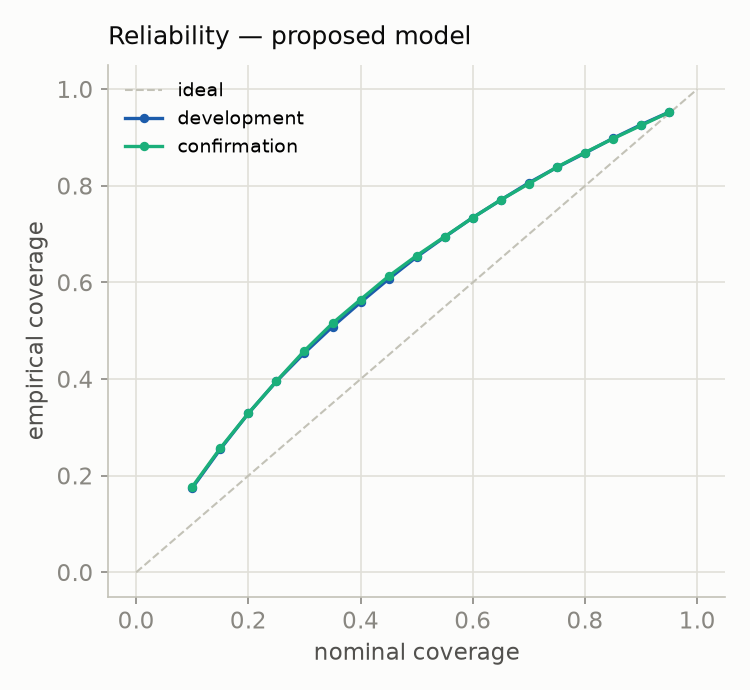
\includegraphics[width=0.62\linewidth]{figures/proposed_reliability.png}
\caption{Reliability of the proposed model, development vs.\ confirmation.}
\label{fig:gp-reliability}
\end{figure}

\begin{figure}[h]\centering
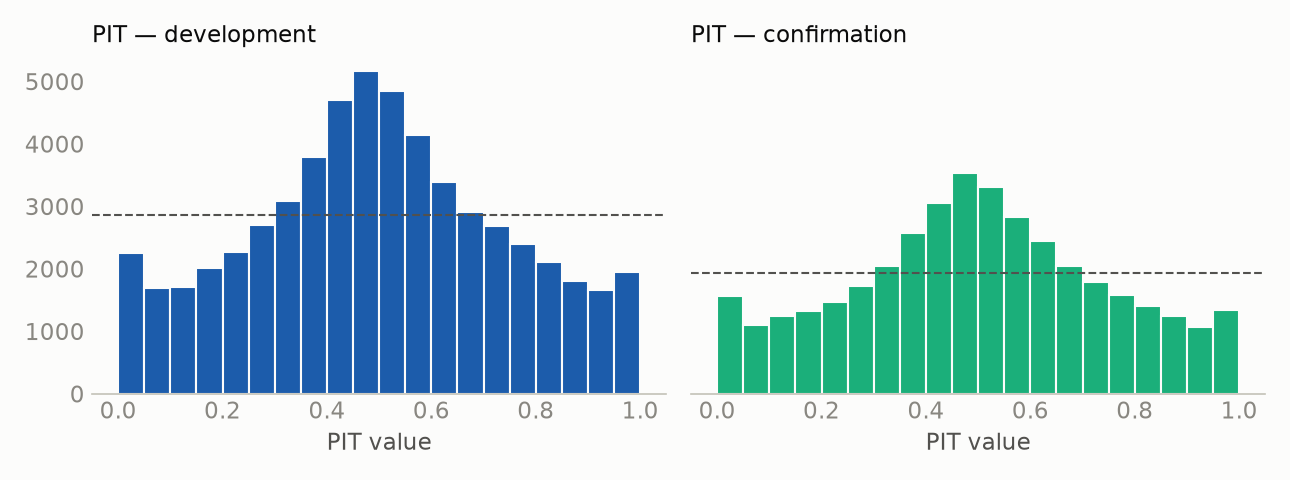
\includegraphics[width=0.9\linewidth]{figures/proposed_pit.png}
\caption{PIT histograms, development vs.\ confirmation (dashed: uniform).}
\label{fig:gp-pit}
\end{figure}

\section{Full development ablation sequence, per channel}
Table~\ref{tab:perchannel-full} extends Table~\ref{tab:perchannel} to every
configuration evaluated on the development set under a single code version.

\begin{table}[h]\centering
\caption{Per-channel RMSE / coverage@0.9, development set, all configurations.
Bold marks the thesis model's row, not the column optimum (individual cells are
edged by specialised variants, e.g.\ corpus-frozen $\tau$ 0.150, harmonic learned graph $v$ 0.071).}
\label{tab:perchannel-full}
\footnotesize
\begin{tabular}{@{}lcccccc@{}}
\toprule
 & \multicolumn{2}{c}{Timing $\tau$} & \multicolumn{2}{c}{Artic.\ $\log r$} & \multicolumn{2}{c}{Velocity $v$} \\
\cmidrule(lr){2-3}\cmidrule(lr){4-5}\cmidrule(lr){6-7}
Configuration & RMSE & cov & RMSE & cov & RMSE & cov \\
\midrule
3 scalar GPs, zero mean      & 0.156 & 0.95 & 0.677 & 0.91 & 0.081 & 0.92 \\
Coregionalized, zero mean                & 0.156 & 0.94 & 0.676 & 0.91 & 0.080 & 0.92 \\
+ features, no graph                   & 0.154 & 0.95 & 0.626 & 0.91 & 0.088 & 0.90 \\
+ features                   & 0.153 & 0.95 & 0.615 & 0.91 & 0.075 & 0.91 \\
+ embeddings, no graph                 & 0.154 & 0.95 & 0.627 & 0.91 & 0.083 & 0.92 \\
\textbf{+ embeddings (proposed model)}       & \textbf{0.152} & 0.95 & \textbf{0.601} & 0.91 & \textbf{0.072} & 0.92 \\
fixed two-stage mean inside the proposed model & 0.158 & 0.94 & 0.652 & 0.91 & 0.080 & 0.91 \\
learned graph               & 0.153 & 0.94 & 0.609 & 0.91 & 0.074 & 0.90 \\
harmonic learned graph       & 0.152 & 0.94 & 0.601 & 0.90 & 0.071 & 0.90 \\
everything               & 0.153 & 0.95 & 0.593 & 0.91 & 0.075 & 0.91 \\
corpus-frozen hyperparameters          & 0.150 & 0.96 & 0.613 & 0.91 & 0.074 & 0.91 \\
frozen + per-piece noise   & 0.151 & 0.97 & 0.613 & 0.91 & 0.075 & 0.94 \\
\bottomrule
\end{tabular}
\end{table}

\section{Why the spectral families tie: the fitted filters}
Figure~\ref{fig:spectral-overlay} makes the kernel-comparison ties
(\S\ref{sec:kernels}) visible. For three development pieces, the full model was
refit once per shape family --- graph Mat\'ern $\alpha \in \{1,2,3\}$ (the
$\alpha{=}1$ member in its additive parameterization) and the heat kernel ---
and the evidence-fitted filters $g(\nu;\hat s)$ overlaid. The families agree
over the low-frequency components, where the prior mass and the smooth
expressive structure live, and disagree only in the mid-tail --- exactly where
the feature kernels and the noise term absorb the variance, so the evidence is
insensitive to the difference. The information is in the graph $\Lg$, not in
the fine shape of the filter.

\figph{spectral_overlay_dev.png}{1.0}{Evidence-fitted spectral filters
$g(\nu;\hat s)$ per kernel family, three development pieces (published anchor
mask, seed 0). Ticks along the base mark each piece's Laplacian eigenvalues.
The families coincide at the low-frequency end and differ only where the
evidence is insensitive, matching the measured statistical
ties.\label{fig:spectral-overlay}}

\noindent Further extended tables (the two-stage development record, the kernel
study's $\mu=0$ block, downstream per-task detail) remain in
the accompanying evidence archive.

% =====================================================================
\begin{thebibliography}{99}
\bibitem{lindgren2011} F.~Lindgren, H.~Rue, J.~Lindstr\"om.
  An explicit link between Gaussian fields and Gaussian Markov random fields:
  the SPDE approach. \emph{JRSS-B}, 2011.
\bibitem{rueheld2005} H.~Rue, L.~Held.
  \emph{Gaussian Markov Random Fields: Theory and Applications}. 2005.
\bibitem{borovitskiy2021} V.~Borovitskiy et al.
  Mat\'ern Gaussian Processes on Graphs. \emph{AISTATS}, 2021.
\bibitem{venkitaraman2018} A.~Venkitaraman, S.~Chatterjee, P.~H\"andel.
  Gaussian Processes Over Graphs. arXiv:1803.05776, 2018.
\bibitem{blancomulero2021} D.~Blanco-Mulero, M.~Heinonen, V.~Kyrki.
  Evolving-Graph Gaussian Processes. \emph{ICML Time Series Workshop}, 2021.
\bibitem{smolakondor2003} A.~J.~Smola, R.~Kondor.
Kernels and regularization on graphs.
In \emph{Learning Theory and Kernel Machines (COLT/Kernel 2003)}, LNCS 2777,
pages 144--158, 2003.
\bibitem{bonilla2008} E.~V.~Bonilla, K.~M.~Chai, C.~K.~I.~Williams.
Multi-task Gaussian process prediction.
In \emph{Advances in Neural Information Processing Systems 20}, 2008.
\bibitem{rubin1976} D.~B.~Rubin.
Inference and missing data.
\emph{Biometrika}, 63(3):581--592, 1976.
\bibitem{nosek2018} B.~A.~Nosek, C.~R.~Ebersole, A.~C.~DeHaven, D.~T.~Mellor.
The preregistration revolution.
\emph{Proc.\ Natl.\ Acad.\ Sci.}, 115(11):2600--2606, 2018.
\bibitem{seashore1936} C.~E.~Seashore (ed.).
\emph{Psychology of the Vibrato in Voice and Instrument}.
University of Iowa Studies in the Psychology of Music, Vol.~III, 1936.
\bibitem{prame1994} E.~Prame.
Measurements of the vibrato rate of ten singers.
\emph{J.\ Acoust.\ Soc.\ Am.}, 96(4):1979--1984, 1994.
\bibitem{prame1997} E.~Prame.
Vibrato extent and intonation in professional Western lyric singing.
\emph{J.\ Acoust.\ Soc.\ Am.}, 102(1):616--621, 1997.
\bibitem{dalessandro1994} C.~d'Alessandro, M.~Castellengo.
The pitch of short-duration vibrato tones.
\emph{J.\ Acoust.\ Soc.\ Am.}, 95(3):1617--1630, 1994.
\bibitem{driedger2016} J.~Driedger, S.~Balke, S.~Ewert, M.~M\"uller.
Template-based vibrato analysis in complex music signals.
In \emph{Proc.\ of the International Society for Music Information Retrieval
Conference (ISMIR)}, pages 239--245, 2016.
\bibitem{ddsp} J.~Engel, L.~Hantrakul, C.~Gu, A.~Roberts.
  DDSP: Differentiable Digital Signal Processing. \emph{ICLR}, 2020.
\bibitem{musictransformer} C.-Z.~A.~Huang et al.
  Music Transformer. \emph{ICLR}, 2019.
\bibitem{remi} Y.-S.~Huang, Y.-H.~Yang.
  Pop Music Transformer (REMI). \emph{ACM MM}, 2020.
\bibitem{oore2018} S.~Oore et al.
  This Time with Feeling: Learning Expressive Musical Performance. 2018.
\bibitem{nanogpt} A.~Karpathy. nanoGPT. \url{https://github.com/karpathy/nanoGPT}.
\bibitem{cancino2018} C.~Cancino-Chac\'on et al.
  Computational Models of Expressive Music Performance: A Review.
  \emph{Front.\ Digit.\ Humanit.}, 2018.
\bibitem{asap} F.~Foscarin et al.
  ASAP: a dataset of aligned scores and performances. \emph{ISMIR}, 2020.
\bibitem{maestro} C.~Hawthorne et al.
  Enabling Factorized Piano Music Modeling with the MAESTRO Dataset.
  \emph{ICLR}, 2019.
\bibitem{vienna4x22} W.~Goebl. The Vienna 4x22 Piano Corpus.
  \emph{Bulletin of the ATR}, 1999.
\end{thebibliography}

\end{document}
